\subsection{Лаборатория инфокоммуникационных технологий}
	
	\subsubsection{Аннотация}

        Курс <<Лаборатория инфокоммуникационных технологий>> получил крайне негативные отзывы. 
                
        Лабораторные работы также нуждаются в серьезной доработке, особенно в части взаимодействия преподавателей со студентами.

        Руководствуясь результатами опроса, Совет студентов и аспирантов ФРКТ выдвигает следующие идеи по улучшению данного курса:
        \begin{enumerate}
            \item сделать четкие критерии получения автомата;
            \item пересмотреть использование Cisco Packet Tracer в связи с уходом компании Cisco из России, вместо этого на занятиях можно
                \begin{itemize}
                    \item рассматривать оборудование компании Huawei;
                    \item перехват различных пакетов с помощью Wireshark;
                    \item сетевые функции Unix систем;
                    \item сетевое программирование (написание программ, использующих сетевые функции операционных систем и т.д.).
                \end{itemize}
            \item заменить преподавателей лабораторных работ на более компетентных и готовых помогать студентам;
            \item сделать курс обязательным только для студентов, чья специализация связана с сетевыми технологиями, а для остальных -- факультативным.
        \end{enumerate}
       

    \subsubsection{Отзыв студентов о лабораторных работах. Преподаватель: Лилеин А.Л. / Щелкунов Н.Н.}
		\begin{figure}[H]
			\centering
			\begin{subfigure}[b]{0.45\textwidth}
				\centering
				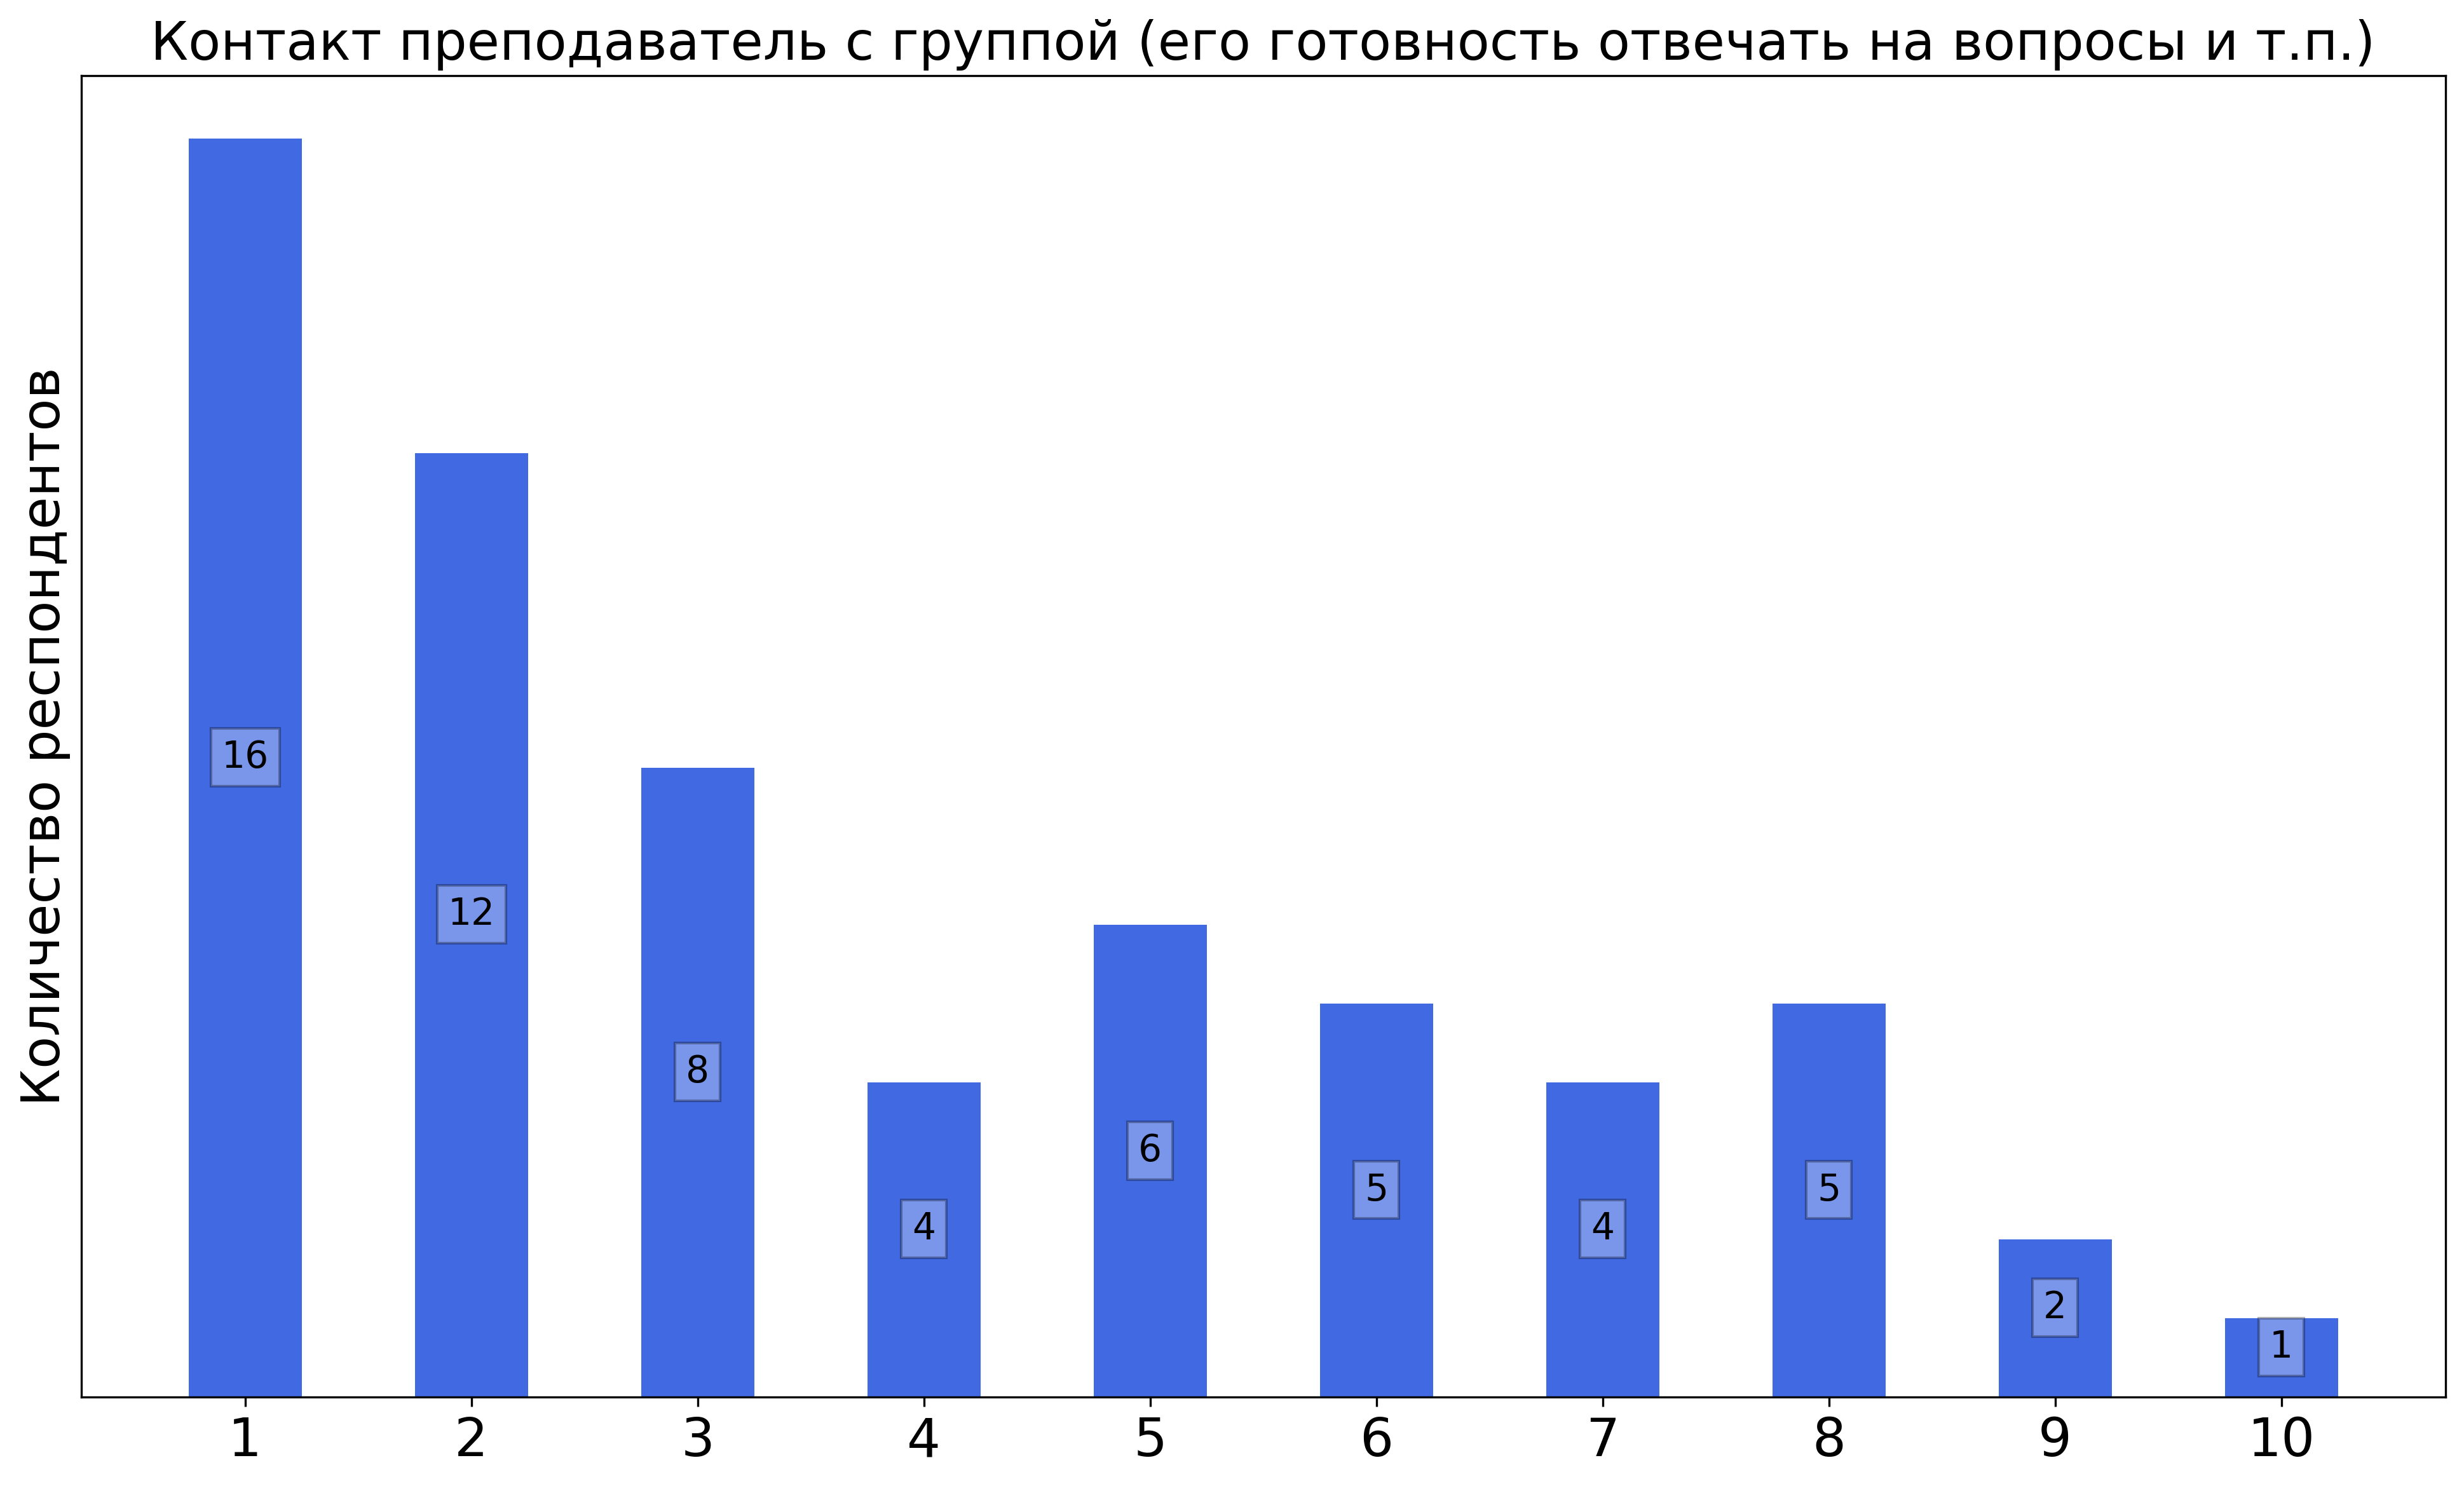
\includegraphics[width=\textwidth]{images/3 course/Лаборатория инфокоммуникационных технологий/labniks-marks-Лилеин А.Л-0.png}
			\end{subfigure}
			\begin{subfigure}[b]{0.45\textwidth}
				\centering
				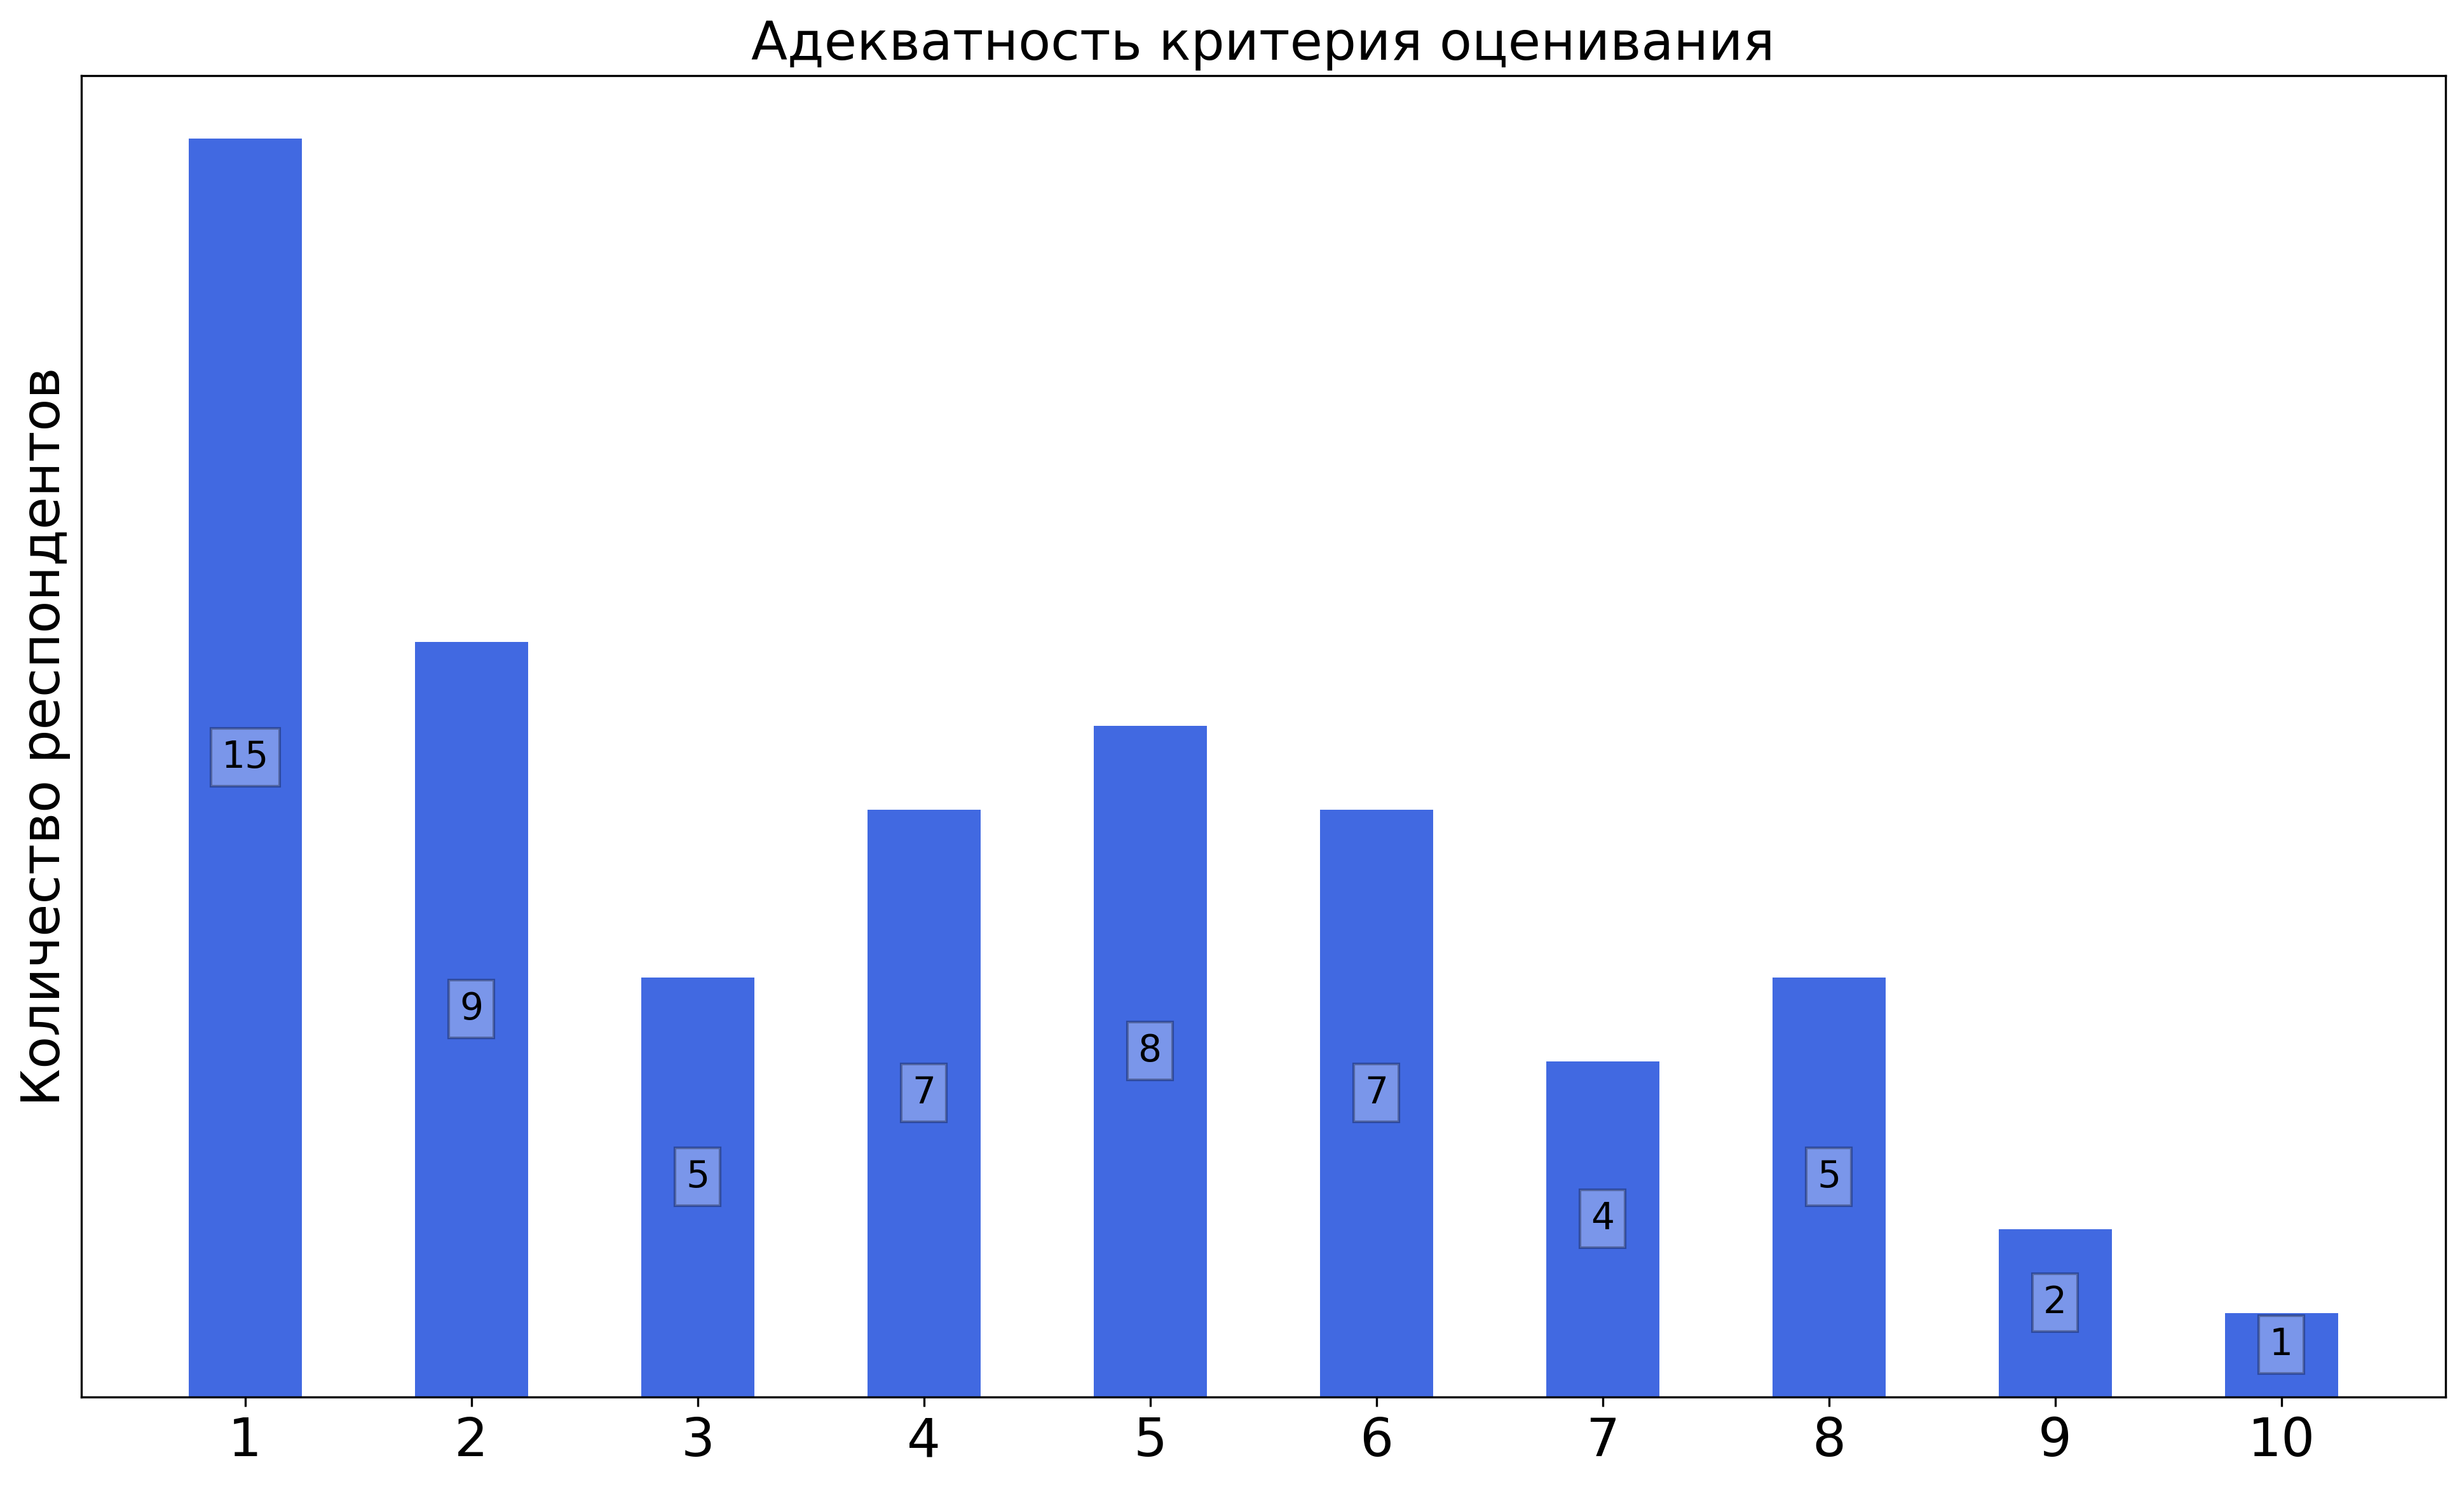
\includegraphics[width=\textwidth]{images/3 course/Лаборатория инфокоммуникационных технологий/labniks-marks-Лилеин А.Л-1.png}
			\end{subfigure}
			\begin{subfigure}[b]{0.45\textwidth}
				\centering
				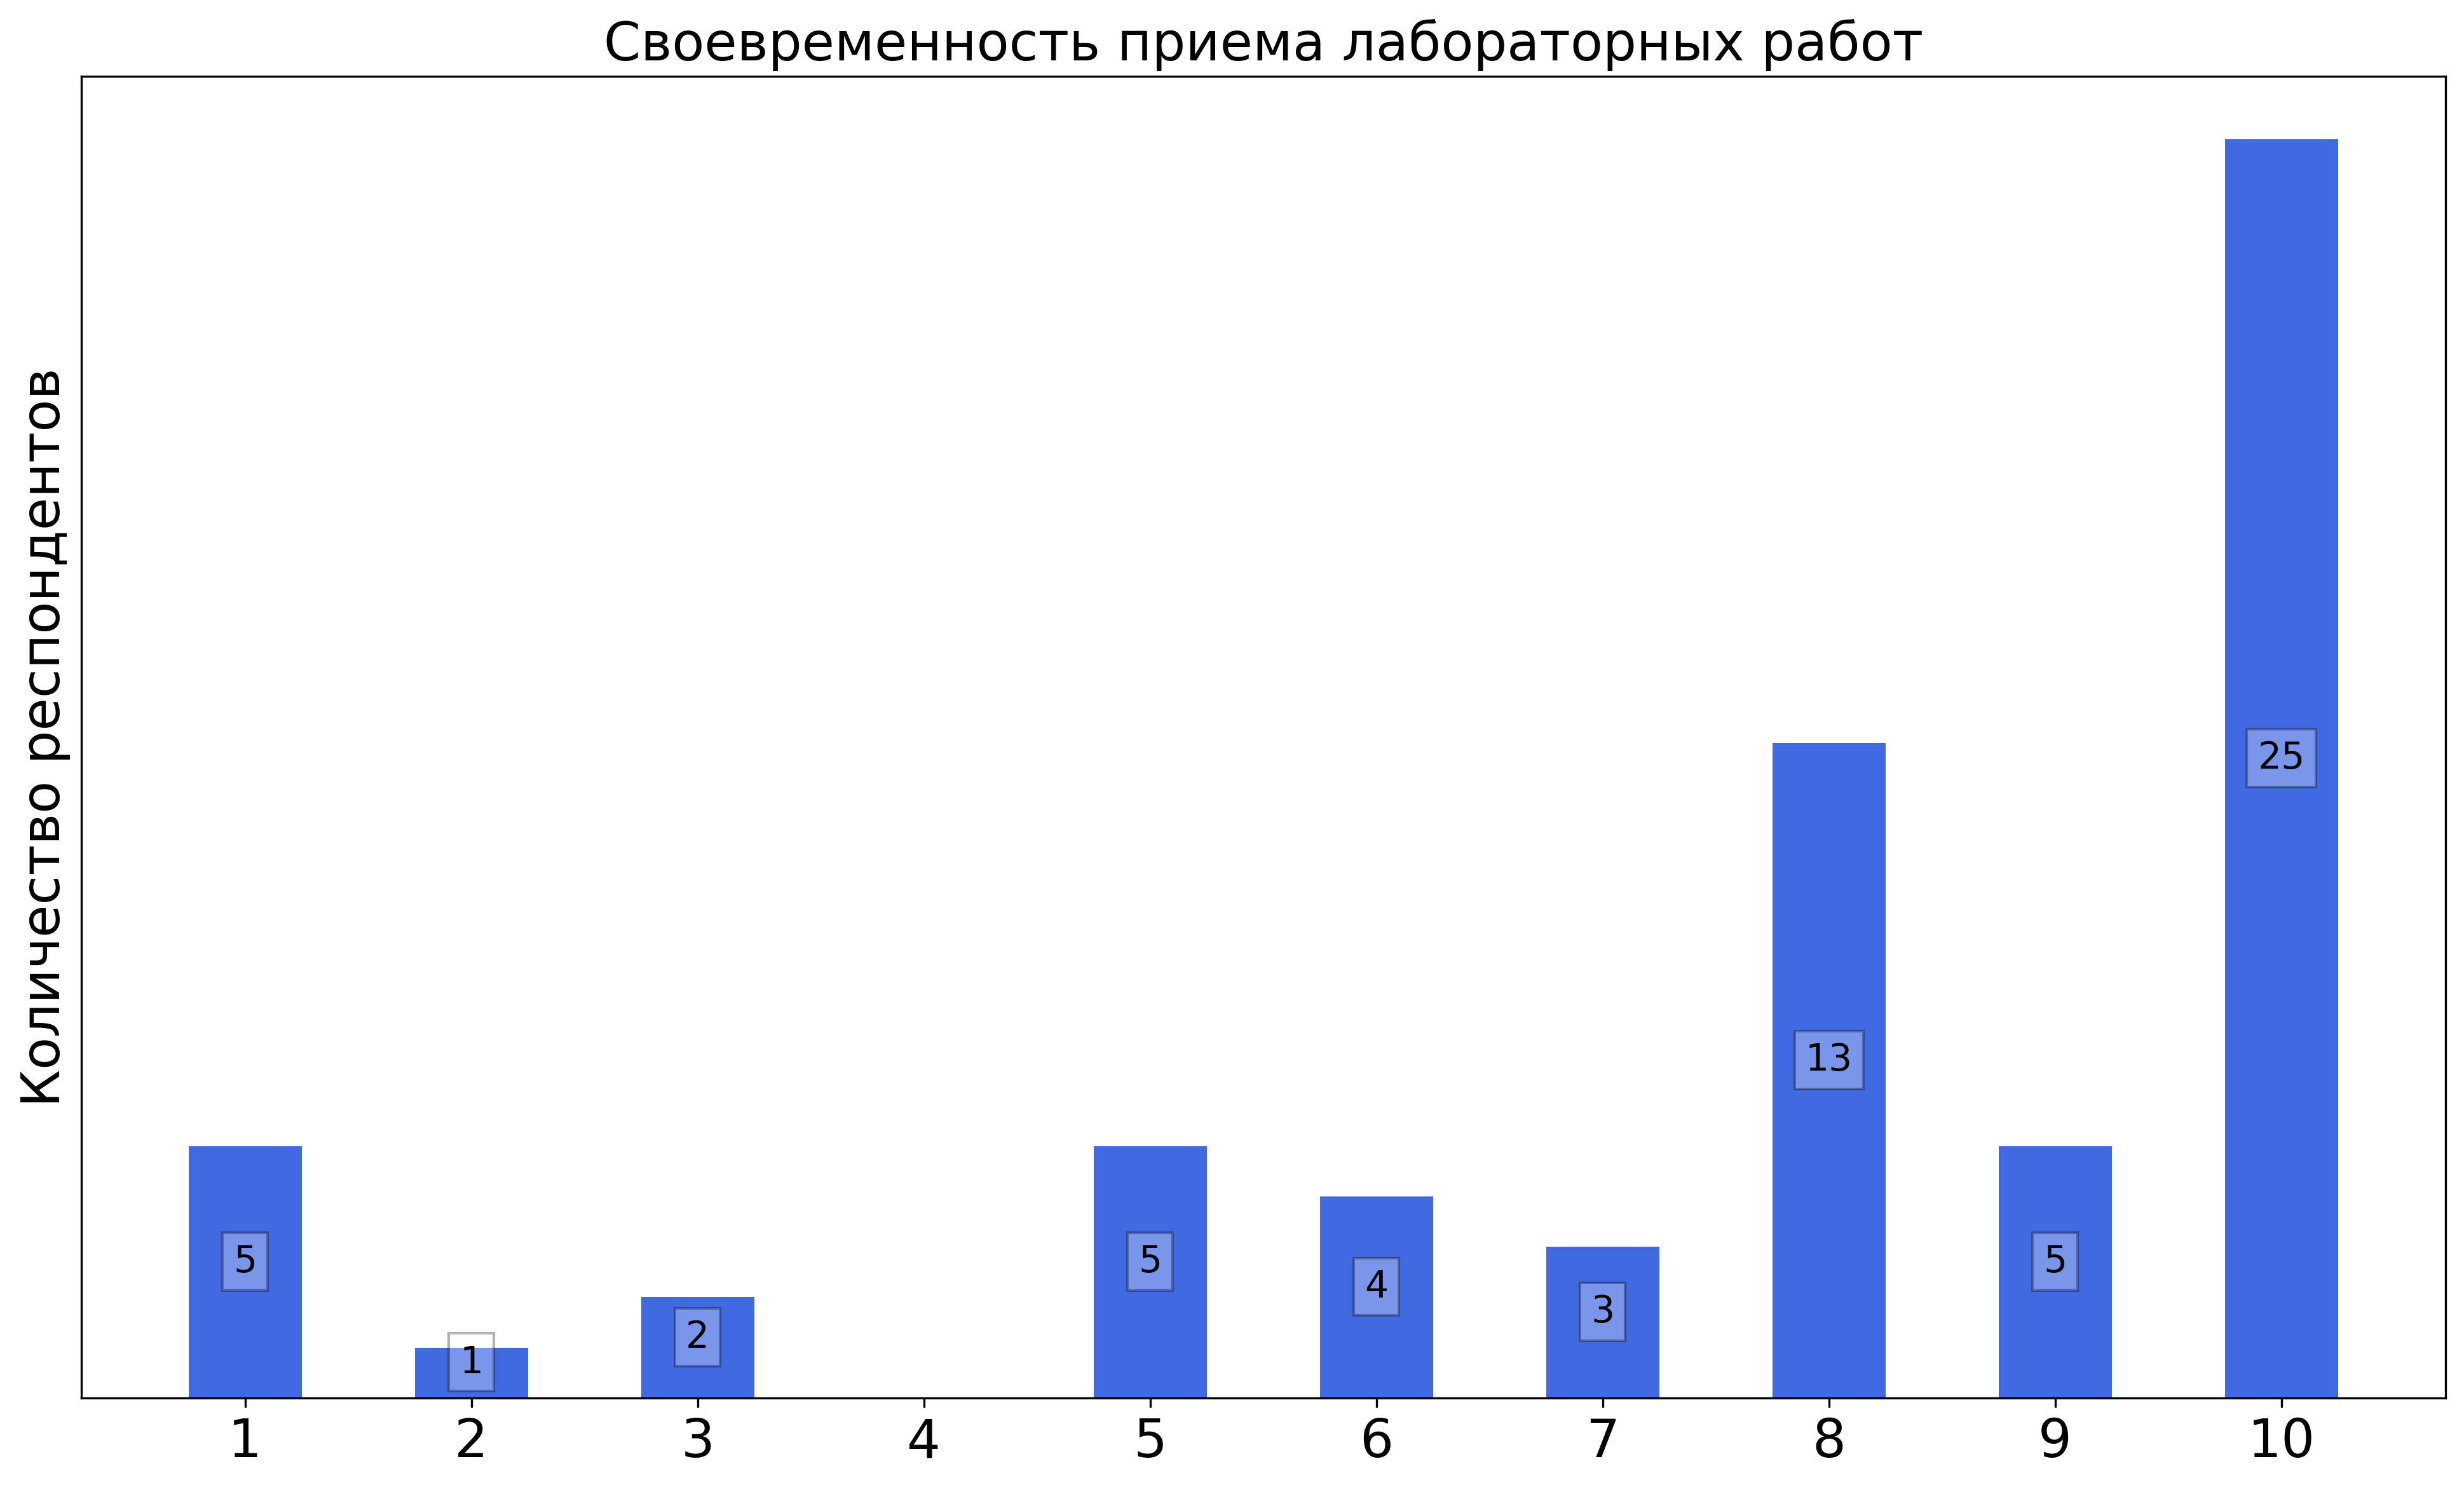
\includegraphics[width=\textwidth]{images/3 course/Лаборатория инфокоммуникационных технологий/labniks-marks-Лилеин А.Л-2.png}
			\end{subfigure}
			\begin{subfigure}[b]{0.45\textwidth}
				\centering
				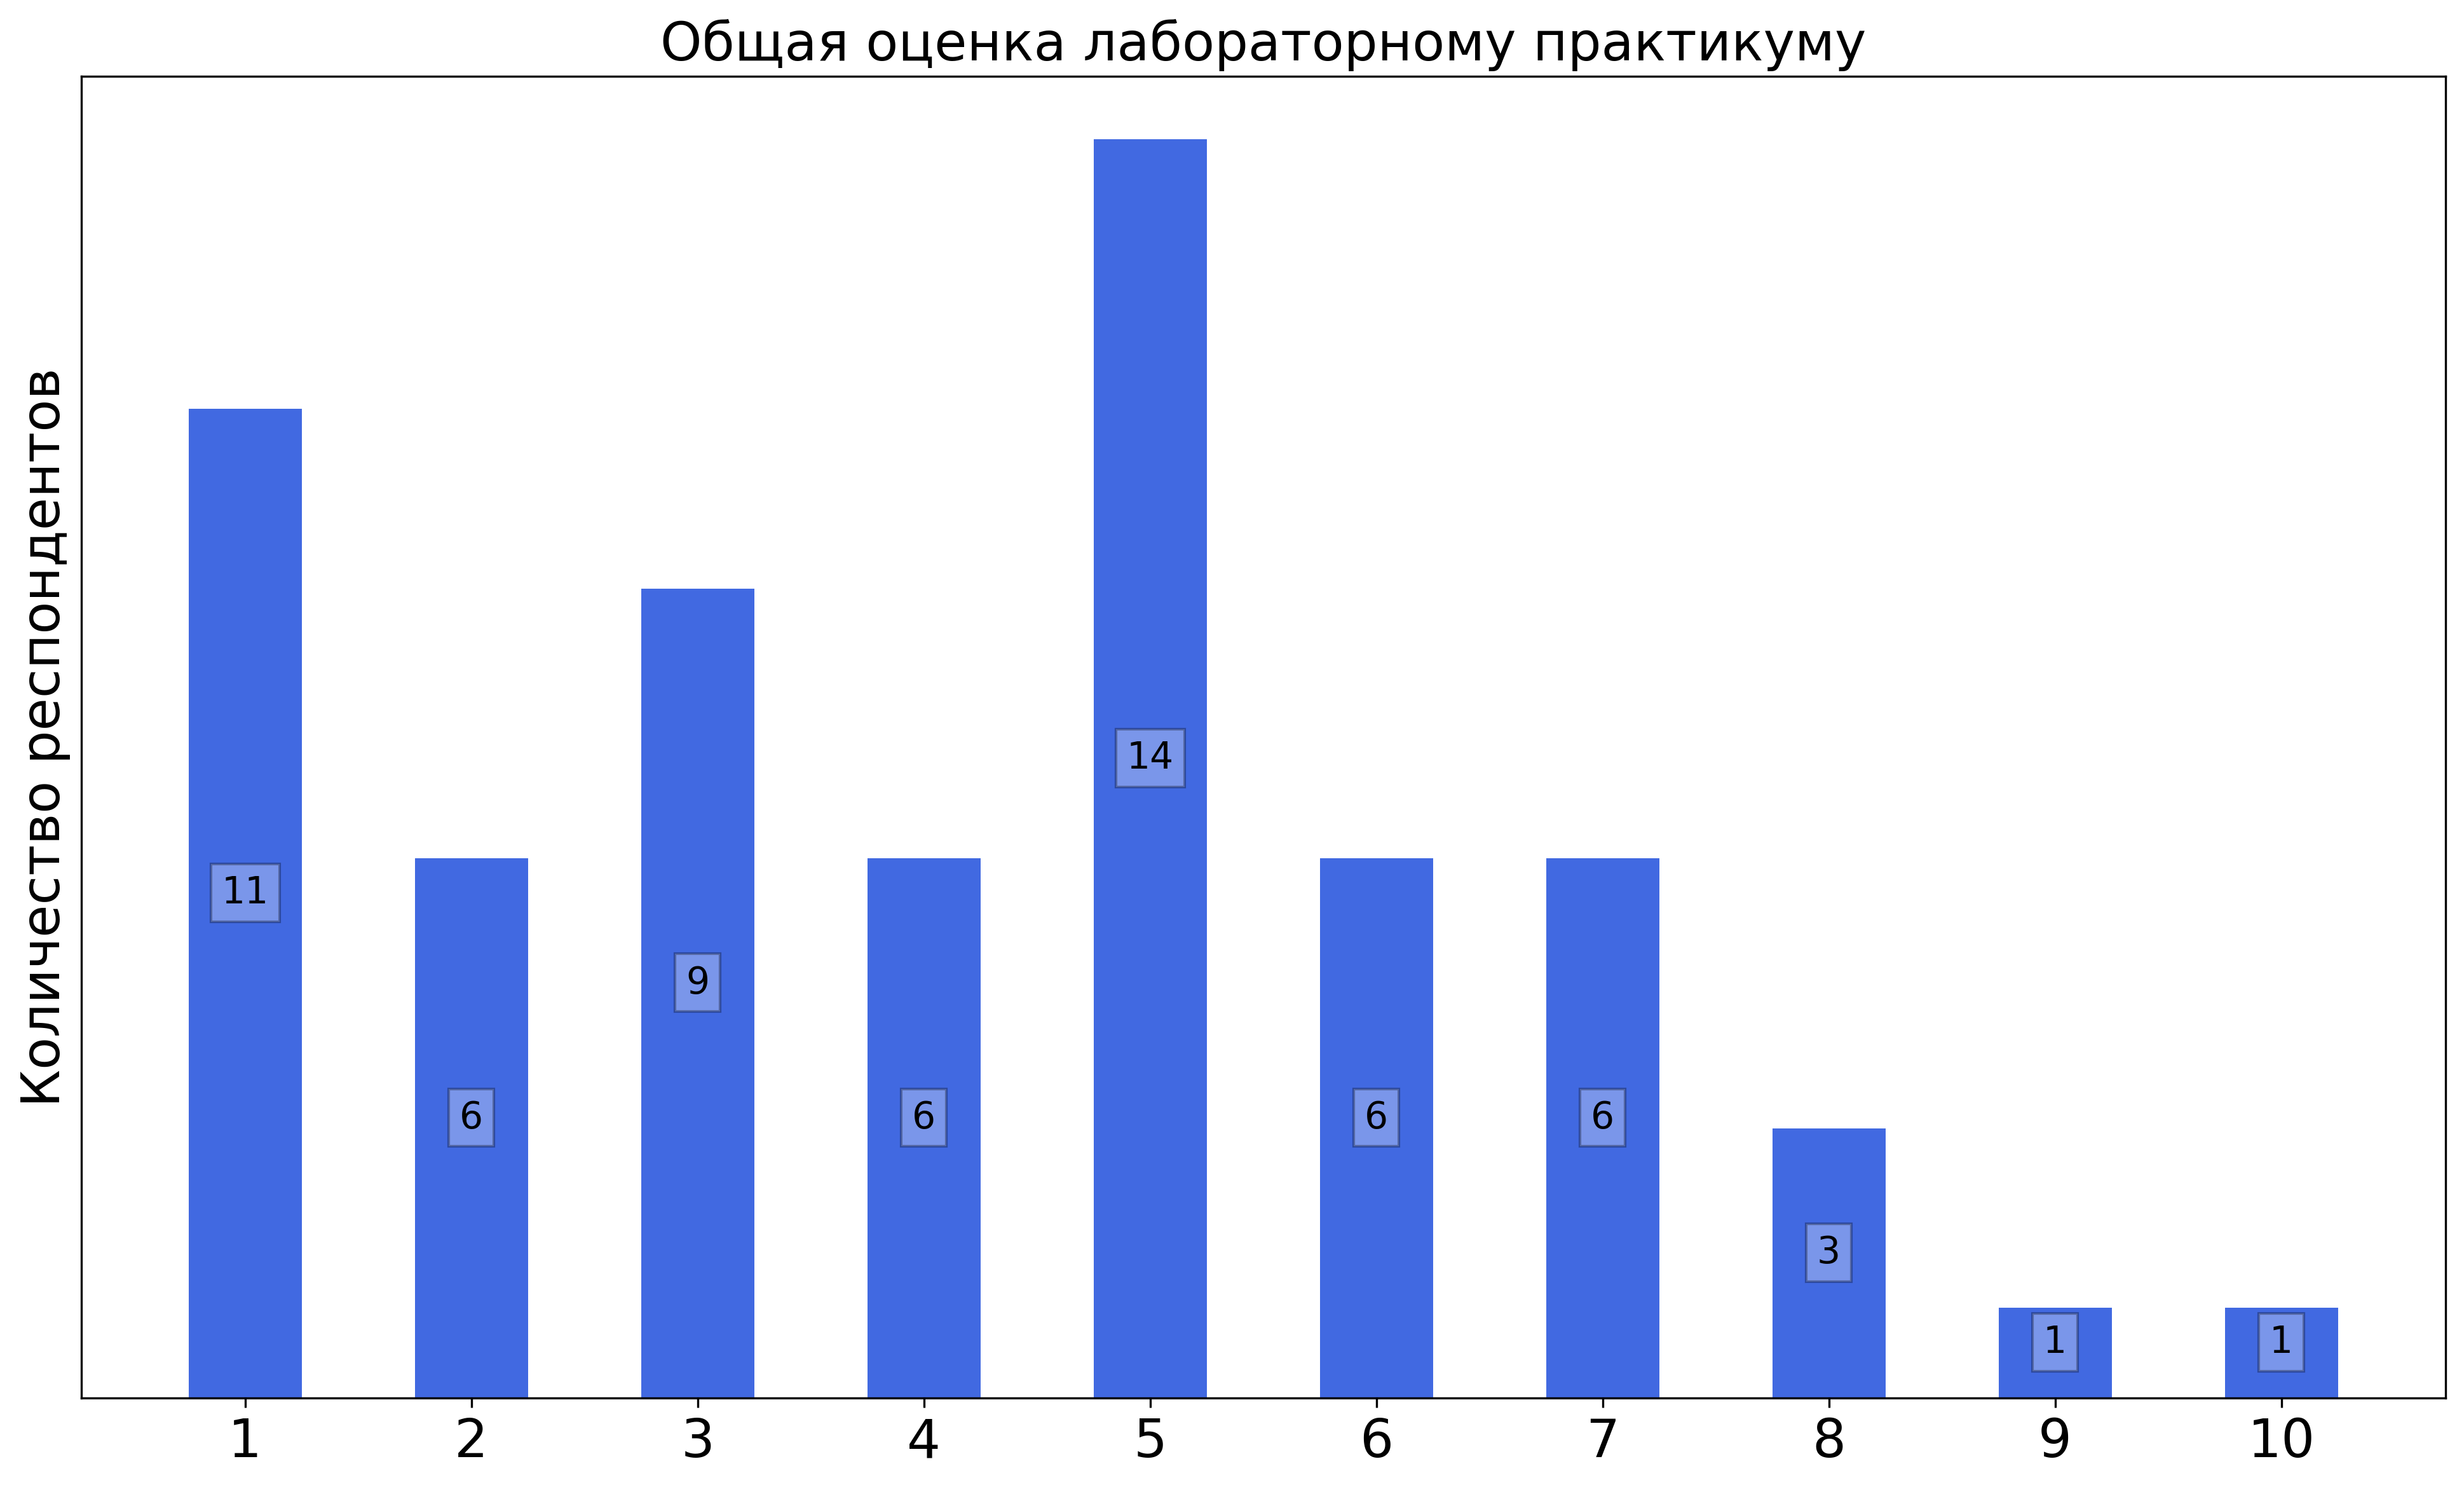
\includegraphics[width=\textwidth]{images/3 course/Лаборатория инфокоммуникационных технологий/labniks-marks-Лилеин А.Л-3.png}
			\end{subfigure}	
			\caption{Оценки респондентов о качестве преподавания лабораторных работ}
		\end{figure}

		\textbf{Комментарии студентов о преподавателе\protect\footnote{сохранены оригинальные орфография и пунктуация}}
            \begin{commentbox} 
                Автоматы получают рандомные люди. Оценка по результатам контрольной выставляется тоже случайным образом. Если что-то не работает, могут с неудом отправить на пересдачу, даже не разбираясь в том, что делал студент. По ощущениям, можно не ходить на эти лабораторные весь семестр, а потом прийти в конце семестра, прочитав какой-то теорминимум и сдавать эти контрольные 
            \end{commentbox} 
       
            \begin{commentbox} 
                Преподаватель, который читает теоретическое введение, готов помогать и отвечать на вопросы. Есть зачем-то еще второй, он приходит через 40 минут и занимается чем-то своим, иногда принимая лабы (проверяет 100\% на экране). Мне на все вопросы отвечал вопросом "А вы как думаете?".

                Ставить автомат/оценки по количеству опозданий на занятия, конечно, бессмыслица, думаю это не надо комментировать. При этом старшекурсники говорят, что те, у кого автомат в осеннем семестре, больше 7 весной не получат. Как это может быть объяснено, тоже не знаю. 
            \end{commentbox} 
       
            \begin{commentbox} 
                Нет четких критериев оценивания. Существуют "автоматы", но выставляются они совершенно непонятным образом. Оценки за контрольные по сетям вообще не учитываются. При выставлении автомата учитывается лишь отсутствие опозданий на занятия, а иногда и вовсе "русская рулетка", что не показывает уровень знаний по предмету.
        
                Стоит обратить внимание, что преподаватель не отвечает на вопросы, а в грубой форме дает понять, что ответа студент не получит. 
            \end{commentbox} 
       
            \begin{commentbox} 
                Печальное зрелище, преподаватели сами не могут ответить на вопрос, если ты парень. В противном случае, иногда все-таки могут.  
            \end{commentbox} 
        
            \begin{commentbox} 
                Странная система оценивания 
            \end{commentbox} 
        
            \begin{commentbox} 
                Странные критерии для получения автомата, мягко говоря - сдать все лабы (это окей), ни одного опоздания и не выходить из аудитории во время рассказа теории 
            \end{commentbox} 
        
            \begin{commentbox} 
                Невозможно получить ответ на вопрос, заданный на лабораторной. Критерии оценки и вовсе плохи, особенно непонятна политика автоматов: их выдают тем, кто ни разу не опаздывал и не пропускал занятия, при этом действительное знание предмета и вовлеченность никак не учитывается. В итоге складывается ситуация, что человек, которые просто приходил вовремя, но ничего не понимает, спокойно уходит с автоматом, но одно опоздание даже по уважительной причине – и приходится писать контрольную, методы оценки которой еще хуже. 
            \end{commentbox} 
        
            \begin{commentbox} 
                Все, кто не получают автомат получают уд.  
            \end{commentbox} 
        
            \begin{commentbox} 
                Отдельно хотелось бы добавить лабы на реальном оборудовании с самого начала, чтобы чуть быстрее понять эволюцию процесса настройки . 
            \end{commentbox} 
        
            \begin{commentbox} 
                Ужасно. Нет слов как ужасно. Лабы это просто выполнение по инструкции лабы(чувствуешь себя обезьяной перепечатывающей инструкцию). Скучно, неинтересно, тупо. +это уже устарело, циско ушло из России и не понятно почему мы учим их систему команд, когда гораздо полезнее было бы учить чтото более общее и приближенное к прикладному программированию(например как на курсе ивт сп фпми) Подача материала ужасная, теоретическая справка в начале лаб подаётся ужасно, непонятно и неинтересно.(преподаватель заикается) 
            \end{commentbox} 
        
            \begin{commentbox} 
                Странное отношение к опоздавшим. На вопросы отвечают нормально.
                Странно делать итоговую оценку по одному финальному тесту. Также тесты бывают сильно неравнозначны по сложности. 
                В целом не очень понятен смысл курса. Нет ощущения применения знаний с лекций Климанова на практике. Ощущение, что курс научил только настраивать современные сети, но не дал более глубокого понимания их работы 
            \end{commentbox} 
        
            \begin{commentbox} 
                Преподаватели не способны ответить на какой-либо вопрос студента, комментируя это тем, что все ответы представлены в презентации на компьютере. 
            \end{commentbox} 
        
            \begin{commentbox} 
                Невнятные и непонятные объяснения, если что-то не работает, то скажут просто это сделать и ничем не помогут
                Невозможно гарантированно получить автомат
                Странные критерии оценивания 
            \end{commentbox} 
        
            \begin{commentbox} 
                Кажется, что этот предмет не помогает лучше понять сети 
            \end{commentbox} 
        
            \begin{commentbox} 
                Разбор команд по презентациям не даёт понимания как настраивается то или иное обородование, а отдача и желание отвечать на вопросы у преподавателей нет. 
            \end{commentbox} 
        
            \begin{commentbox} 
                Сама программа потрясающая, но ее не раскрывают даже на половину. Преподаватели вообще не пытаются помочь, создается ощущение, что они либо вообще не хотят помогать, либо не знают, как работать в этой программе. Но к их теоретическим знаниям вопросов нет 
            \end{commentbox} 
        
            \begin{commentbox} 
                Никакой помощи от преподавателей на лабораторных работах, на любой вопрос огрызаются и посылают читать методичку к работе. Ощущается, как будто сами преподаватели плохо знают курс, так как некоторые студенты загоняли в угол обычными вопросами про Лаборатория инфокоммуникационных технологий.

                Контрольная в конце семестра вообще не имеет никаких критериев оценки, можно сделать 80\% работы и получить уд3, как и человек который сдавал первым и не сделал ничего. Почти вся группа получила тройки, хотя задание у многих было выполнено 
            \end{commentbox} 
        
            \begin{commentbox} 
                Достаточно часто преподователи по лабам (все трое). Вместо того, чтобы ответить на вопрос и помочь разобраться, говорят "ищите ответ в презентации". За счёт чего падает мотивация пытаться разабраться в лабе  
            \end{commentbox} 
        
            \begin{commentbox} 
                Предмет и в целом лабораторные - интересные. НО ужасный контакт с аудиторией, нежелание отвечать на вопросы убивает всё желание изучать предмет. На контрольной получил в качестве задачи схему с аппаратурой, котороя была рассмотрена всего один раз в середине семестра и потом не использовалась. Никто из группы не вспомнил, что с ней делать и оценки разделились на два типа: неуд (верные шаги к решению никак не оценивались) и уд 3 (его получили люди, которые догадались, что если НИЧЕГО не сделать, на самом деле один ПК пингуется и так - им поставили 3 с минусом).  
            \end{commentbox} 
        
            \begin{commentbox} 
                Весёлые деды, которые как и Климанов не слышали про уважение студентов. Хорошо, что любят девушек и ставят автоматы, только благодаря этому осилила данный курс))) 
            \end{commentbox} 
        
            \begin{commentbox} 
                Я не понимаю, почему я прохожу курс Cisco-лаб и изучаю то, что специфично для Cisco, хотя они ушли из России.
        
                Лектор читает материал с презентаций, его невозможно слушать - ты сразу засыпаешь. Невероятно скучно. Я жалею, что тратил время на это. 
            \end{commentbox} 
        
            \begin{commentbox} 
                Худший курс, который у меня был на физтехе. Этот предмет опускает наш вуз на уровень региональной шараги. 
        
                Полностью потеряна связь между студентами и преподавателями. Это похоже не на обучение, а на выход на прогулку в тюрьме. «Во столько-то приди, столько-то сдай, сюда не ходи, это не спрашивай, здесь постучи по клавиатуре для виду, не понятно - открой кривые презентации, их явно методисты писали»
                
                Короче, преподы, которые требуют дисциплины и формального отношения, а не знаний предмета, это явно не про физтех 
            \end{commentbox} 
        
            \begin{commentbox} 
                Лабы как лабы. В целом всё хорошо. 
            \end{commentbox} 
        
            \begin{commentbox} 
                Здесь, к сожалению, также весьма грубое отношение к студентам, но добавляется еще следующий момент: если что-то не получается в лабораторной работе, то преподаватель на просьбу о помощи скажет посмотреть презентации (однако на студенческих компьютерах они неполные!), а никаких существенных Советов не даст. Самое обидное, что в случае одного такого прокола (то есть к концу занятий вы не справились до конца), вы точно не получите автомат (им важно только, чтобы у вас было 100\%, все остальное не волнует). Насчет грубости, которая лучше всего проявляется на контрольных работах: при проверке вам категорически запрещается говорить, а при любой попытке объяснить своё решение вас оборвут словами: «Помолчите, пожалуйста!». Оценивание тоже непонятно как происходит (система внутренняя пятибалльная): все правильно - 5, что-то неправильно - 3, иногда 4- (обычно когда что-то неправильно, но им очень понравилось, как все остальное сделано). Причём заранее критерии неизвестны. 
            \end{commentbox} 
        
            \begin{commentbox} 
                Курс плох, во время проведения лабораторных работ нет никакой помощи от преподавателей и получается так, что приходится нужную информацию искать в интернете, В основном ничего не понятно. В начале пары преподаватель просто читает презентацию, что не особо помогает в лабораторных работах. Система оценивания - ужасна. Как я понял существуют 3 оценки, неуд 2, уд 3(если есть ошибки) и отл 8 если всё идеально без ошибок, что необъективно 
            \end{commentbox} 
        
            \begin{commentbox} 
                Заикающийся преподаватель по 40 минут зачитывает слайды с презентации и не может ответить почти ни на один вопрос студентов. После чего самостоятельное выполнение лабораторных работ в ПО Cisco. После контрольной работы преподавателем на мою просьбу объяснить, чего мне не хватило до полной работы схемы (позже выяснилось, что одной простой команды) было заявлено, что у него нет цели меня чему-то научить, ему нужно только проверить мои знания. 
            \end{commentbox} 
        
            \begin{commentbox} 
                Преподаватель почти никогда не может помочь с выполнением работы. Делает это очень неохотно. Автоматы раздали по непонятному принципу, так в моей группе их почему-то вообще никто не получил.  
            \end{commentbox} 
        
            \begin{commentbox} 
                Курс ужасен со всех точек зрения, фактически, он и вовсе нужен только кафедре ИСС, у которой ведётся усложнённый курс. В начале лабораторной работы монотонно зачитывается теория из методички, слушать которую очень тяжело, ибо лектор из преподавателя крайне посредственный. При выполнении лабораторной работы преподаватели вообще не помогают понять, что не так, видно, что они абсолютно не заинтересованы в том, чтобы чему-либо научить. Как правило, они просто говорят подумать самому, что пошло не так, и не помогают решить проблему. Весь контроль заключается в том, что преподаватель смотрит, что в лабе счётчик выполнения дошёл до 100\%, при этом если у студента чего-то не получается, они не пытаются научить, а просто игнорируют проблему. По итогу можно сказать, что студенты сами осваивают курс по решениям лабораторных из интернета, ибо всё, что делают преподаватели, - это простая фиксация заветных 100\% на экране. Итоговая контрольная и вовсе очень странная, приходится решить задачу с нуля, чего никогда не происходит на лабораторных работах, из-за чего с ней возникают трудности. Если же задачу решить не удалось, студенту не объясняют, что не так, говоря, что задачи из контрольных не предназначены для разбора. В общем, курс вызывает самые неприятные впечатления. На мой взгляд, это вообще самый худший предмет на 3 курсе. Абсолютно халатное отношение преподавателей к своему делу в совокупности с полной бесполезностью курс для всех, кто его проходит (речь именно о базовом курсе для большинства студентов) и методике оценивания в формате, которому не обучают в течение семестра, вызывает исключительно негативное впечатление.  
            \end{commentbox} 
        
            \begin{commentbox} 
                Ужасный практикум по компьютерным сетям. Преподаватели разговаривают со студентами на повышенных тонах, на вопросы по материалу ответить не могут, часто отвечают фразами по типу "вы сюда зачем пришли вообще?". Теория лабораторных зачитывается по слайдам и дальше никак не поясняется, что делает почти невозможным самостоятельное выполнения лабораторной. Так как лабораторная зависит от программы-симулятора, происходят иногда сбои или такие случаи, что программа не засчитывает 1-2\% выполнения лабораторной и по окончании времени практикума за неё ставится '-' без пояснений как решить проблему, что приводит к сгоранию автомата. К сгоранию автомата также приводит опоздание на минуту или какой-то ещё малейший проступок. В конце семестра проводится контрольная не соответствующая сложности курса, на которой преподаватель вечно ругается и ставит тройку за малейшие недочеты. 
            \end{commentbox} 
        
            \begin{commentbox} 
                Для того чтобы сдавать работы необходимо просто переписывать команды из решения лабораторных работы, в ином случае невозможно успеть выполнить требуемые работы, из-за впервые увиденного и большого количества материала. 
            \end{commentbox} 
        
            \begin{commentbox} 
                Токсичный мерзопакостный старикашка. Система выдачи автоматов - это вообще смех. А нарастающая сложность контрольных - убийство 
            \end{commentbox} 
        
            \begin{commentbox} 
                На вопросы отвечать не готовы. Говорят, посмотрите в check-results. 
            \end{commentbox} 
        
            \begin{commentbox} 
                Напряжённая атмосфера, иногда даже вопросы некомфортно задавать, очень формальные критерии оценивания, выставления "автоматов" и т д.. Но понрпвились презентации перед началом самих практических работ, это полезно. 
            \end{commentbox} 
        
            \begin{commentbox} 
                Критерии автомата не известны, но вопросы очень сложно добиться внятного ответа. 
            \end{commentbox} 
        
            \begin{commentbox} 
                Наиглупейшая система оценивания. В конце семестра часть группы пишет кр, а другая уходит с автоматами. Кто куда попадёт решается исключительно опозданиями и алфавитным порядком фамилий. 
        
                Я попал писать контрольную, нам дали задачу которую НИКТО из группы НЕ РЕШИЛ, однако некоторым ставили уд3. И ладно бы за старания (объяснить что делал), но нет, препод доверяет только чиселкам в компьютере, показывает 0\% => ничего не делал. Учитывая что это сети и всё может сломаться даже если частично работало.
                После этого я переписал контрольную с более адекватной задачей.
        
                Система со случайно выпадающими задачами требует досконально знать весь пройденный материал. Такая система уместна на устном экзамене основных предметов вроде матана, но Лаборатория инфокоммуникационных технологий таковым не являются. 
            \end{commentbox} 
        
            \begin{commentbox} 
                Циско деды плохи, иногда не могут объяснить то, что происходит. Выгоняют до конца пар, потому что "хотят есть", но если опаздал хотя бы на минуту, то это сразу невозможность получить автомат. Двойные стандарты. 
            \end{commentbox} 
        
            \begin{commentbox} 
                Лабораторные работы не дают глубокого понимания, так как всё сводится к перекликиванию методички, хотелось бы более "самостоятельных" работ для лучшего условения (возможно, в другом симуляторе). 
        
                Странные критерии оценивания - непрозрачная система автоматов, основанная на количестве опозданий, при этом могут кому-то дать автомат и кому-то - нет при одинаковых количествах опозданий.  Так же на контрольной страшивают с разной строгостью, видимо тоже зависит от опозданий. Хотелось бы прозрачности и равноправия в этих вопросах. 
            \end{commentbox} 
        
            \begin{commentbox} 
                Очень бесполезно, всю пару сидим и просто выполняем задание в PacketTracer. Это не дает абсолютно никаких знаний, просто ctrl c ctrl v из условий задания в приложение 
            \end{commentbox} 
        
            \begin{commentbox} 
                То, что автоматы выдаются по количеству опозданий, говорит само за себя. Хотя лабники иногда объясняют нормально, если сспрашивать 
            \end{commentbox} 
        
            \begin{commentbox} 
                Мне,  кажется, что за две пары можно было рассказать намного больше. Не дает никаких указаний по лабораторной. Рассказывает по cisco презентациям. На ютубе можно найти преподователей/профыесоров (которых приходится смотреть из-за нехватки объяснений нащего преподователя) из Индии, которые на английском рассказывают те же презентации намного подробнеене.  Не приводит примеры в packet tracer , хотелось бы что хоть что-то : базовые элементы управления , пояснения где что находится, как открыть командную строку на том или ином устройстве, и примеры схем , чтобы можно было видеть как все работает, а не просто исходить из картинок в презентации. Сравнивал , что преподают у нас и в группе у Климанова(рассказывали и показывали материалы друзья). Там Максим  Михайлович ведет прямо настоящие семинары со своими презентациями и примерами решения задач, это хорошо дополняет лекции, а у нас преподователь только лишь ссылается на них. 
            \end{commentbox} 

    \subsubsection{Отзыв студентов о лабораторных работах. Группа NetCracker}
        \begin{figure}[H]
            \centering
            \begin{subfigure}[b]{0.45\textwidth}
                \centering
                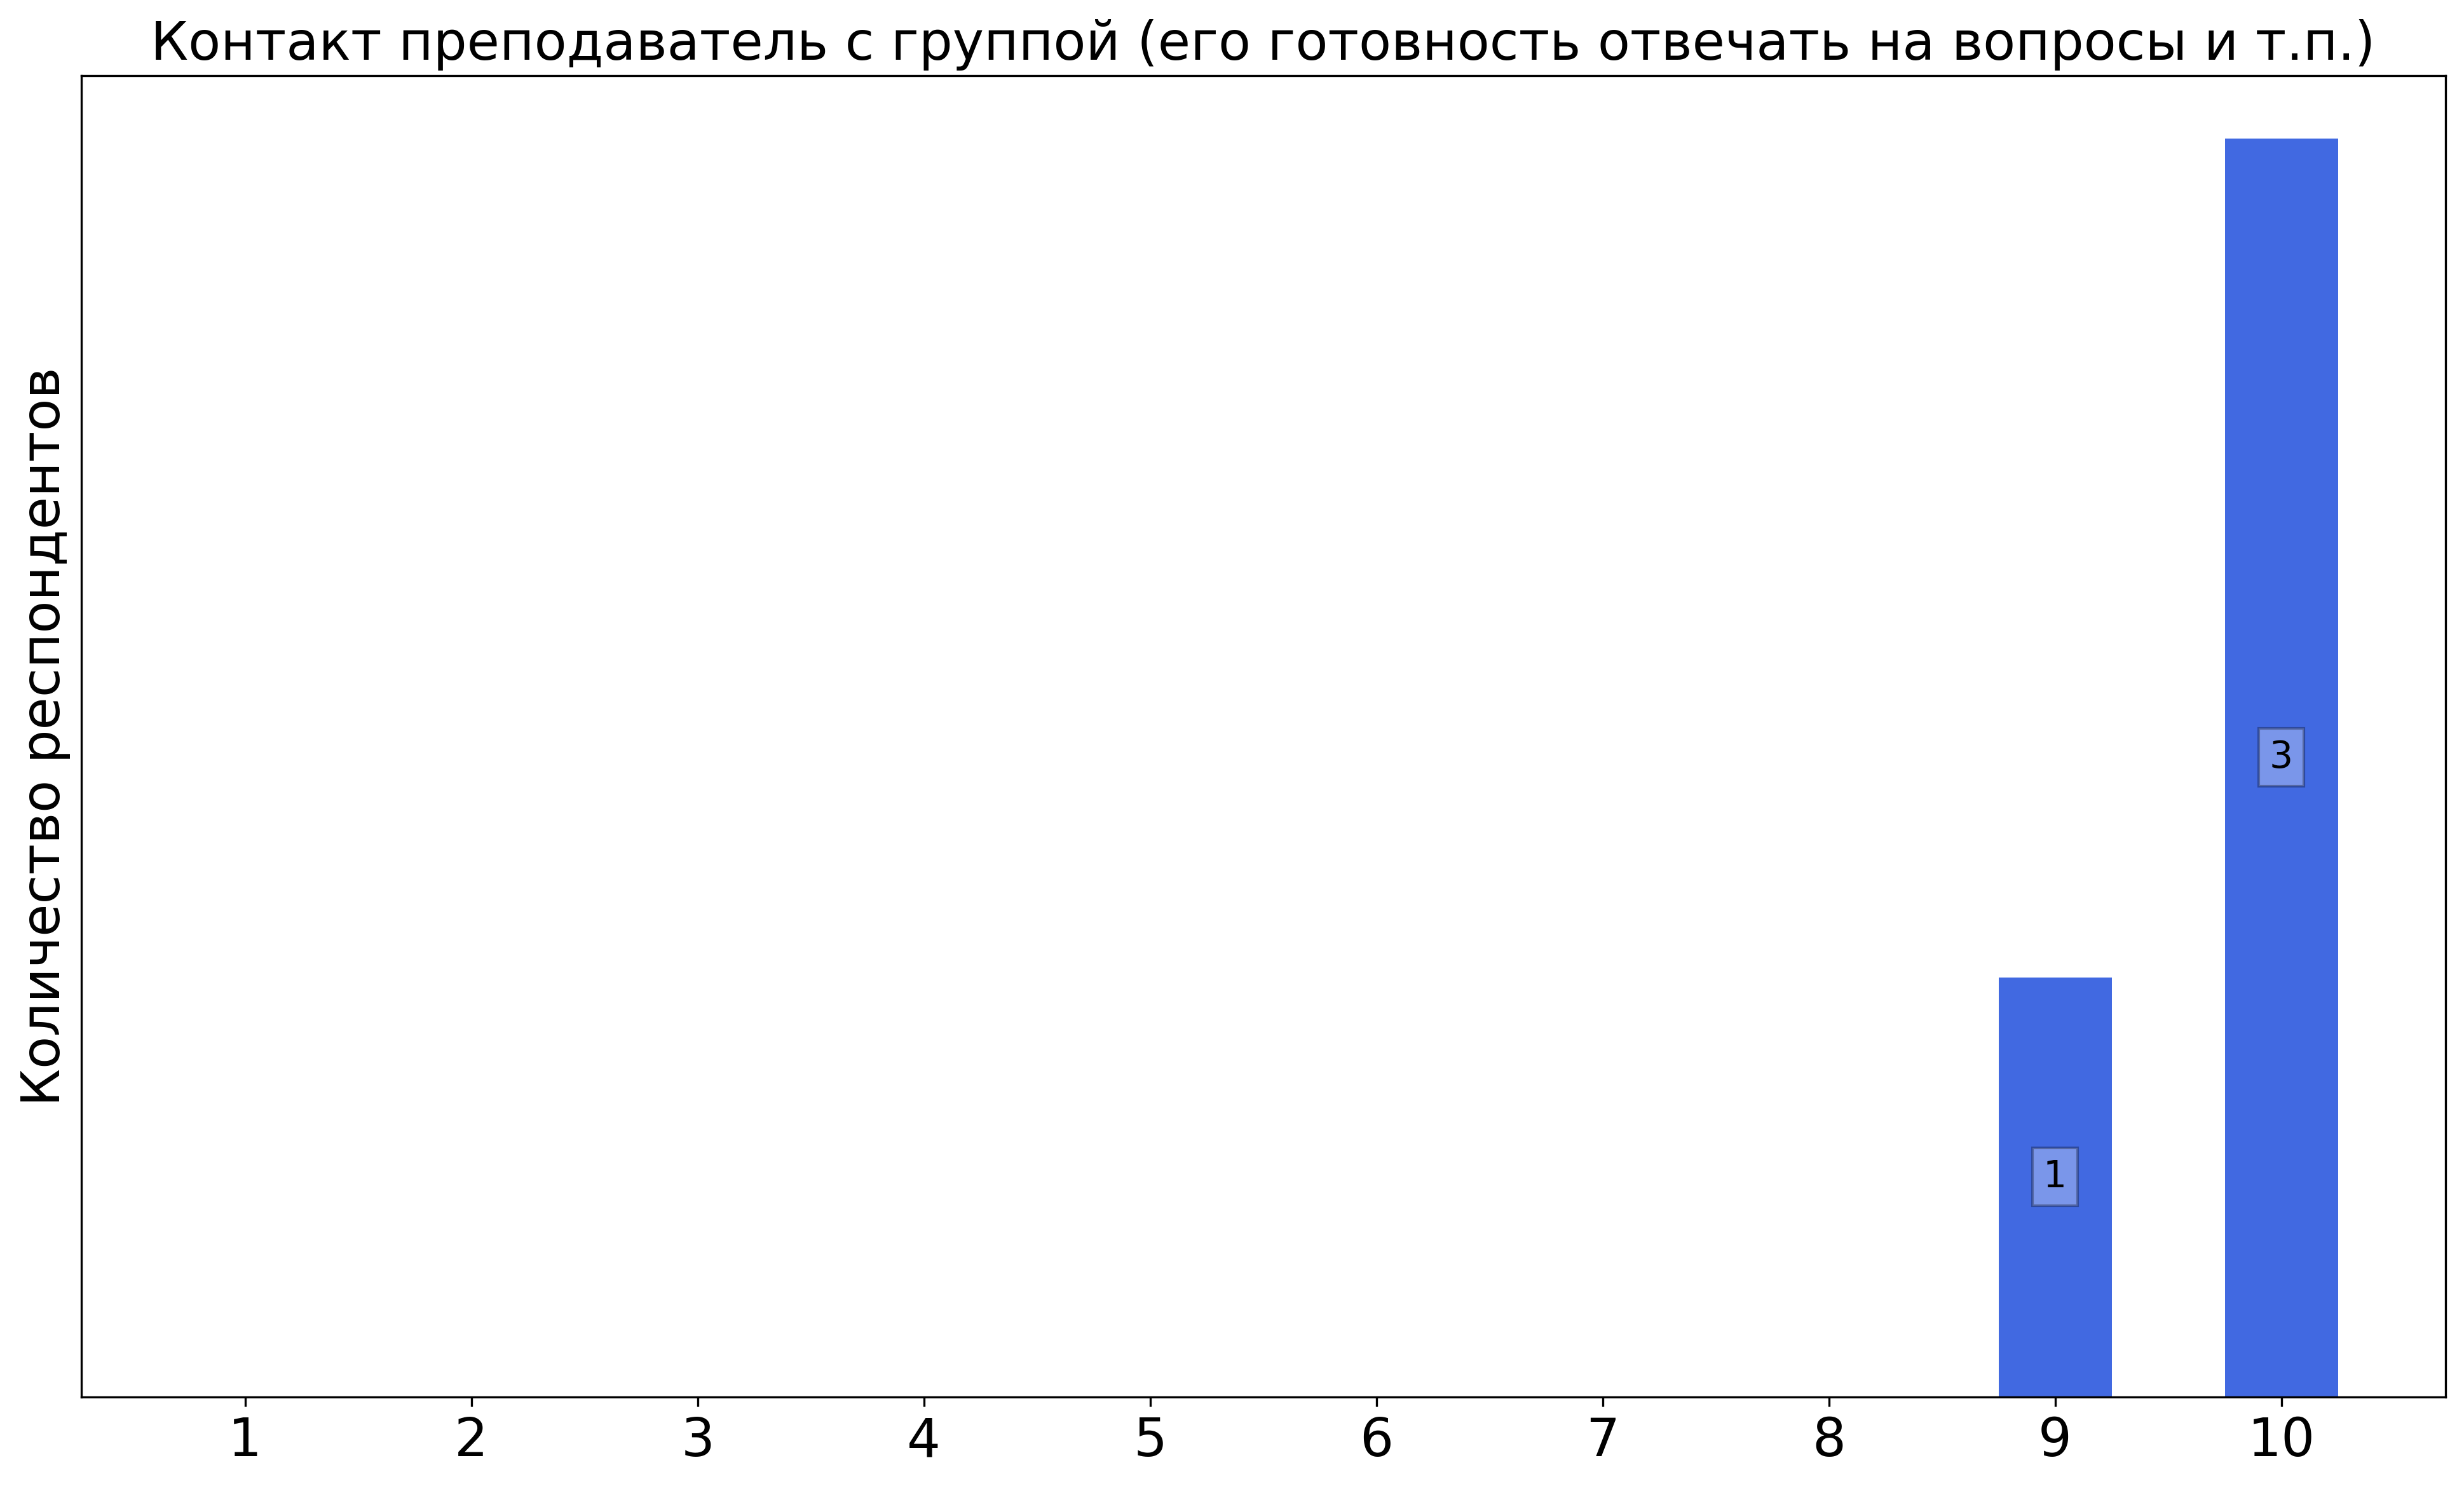
\includegraphics[width=\textwidth]{images/3 course/Лаборатория инфокоммуникационных технологий/labniks-marks-NetCracker-0.png}
            \end{subfigure}
            \begin{subfigure}[b]{0.45\textwidth}
                \centering
                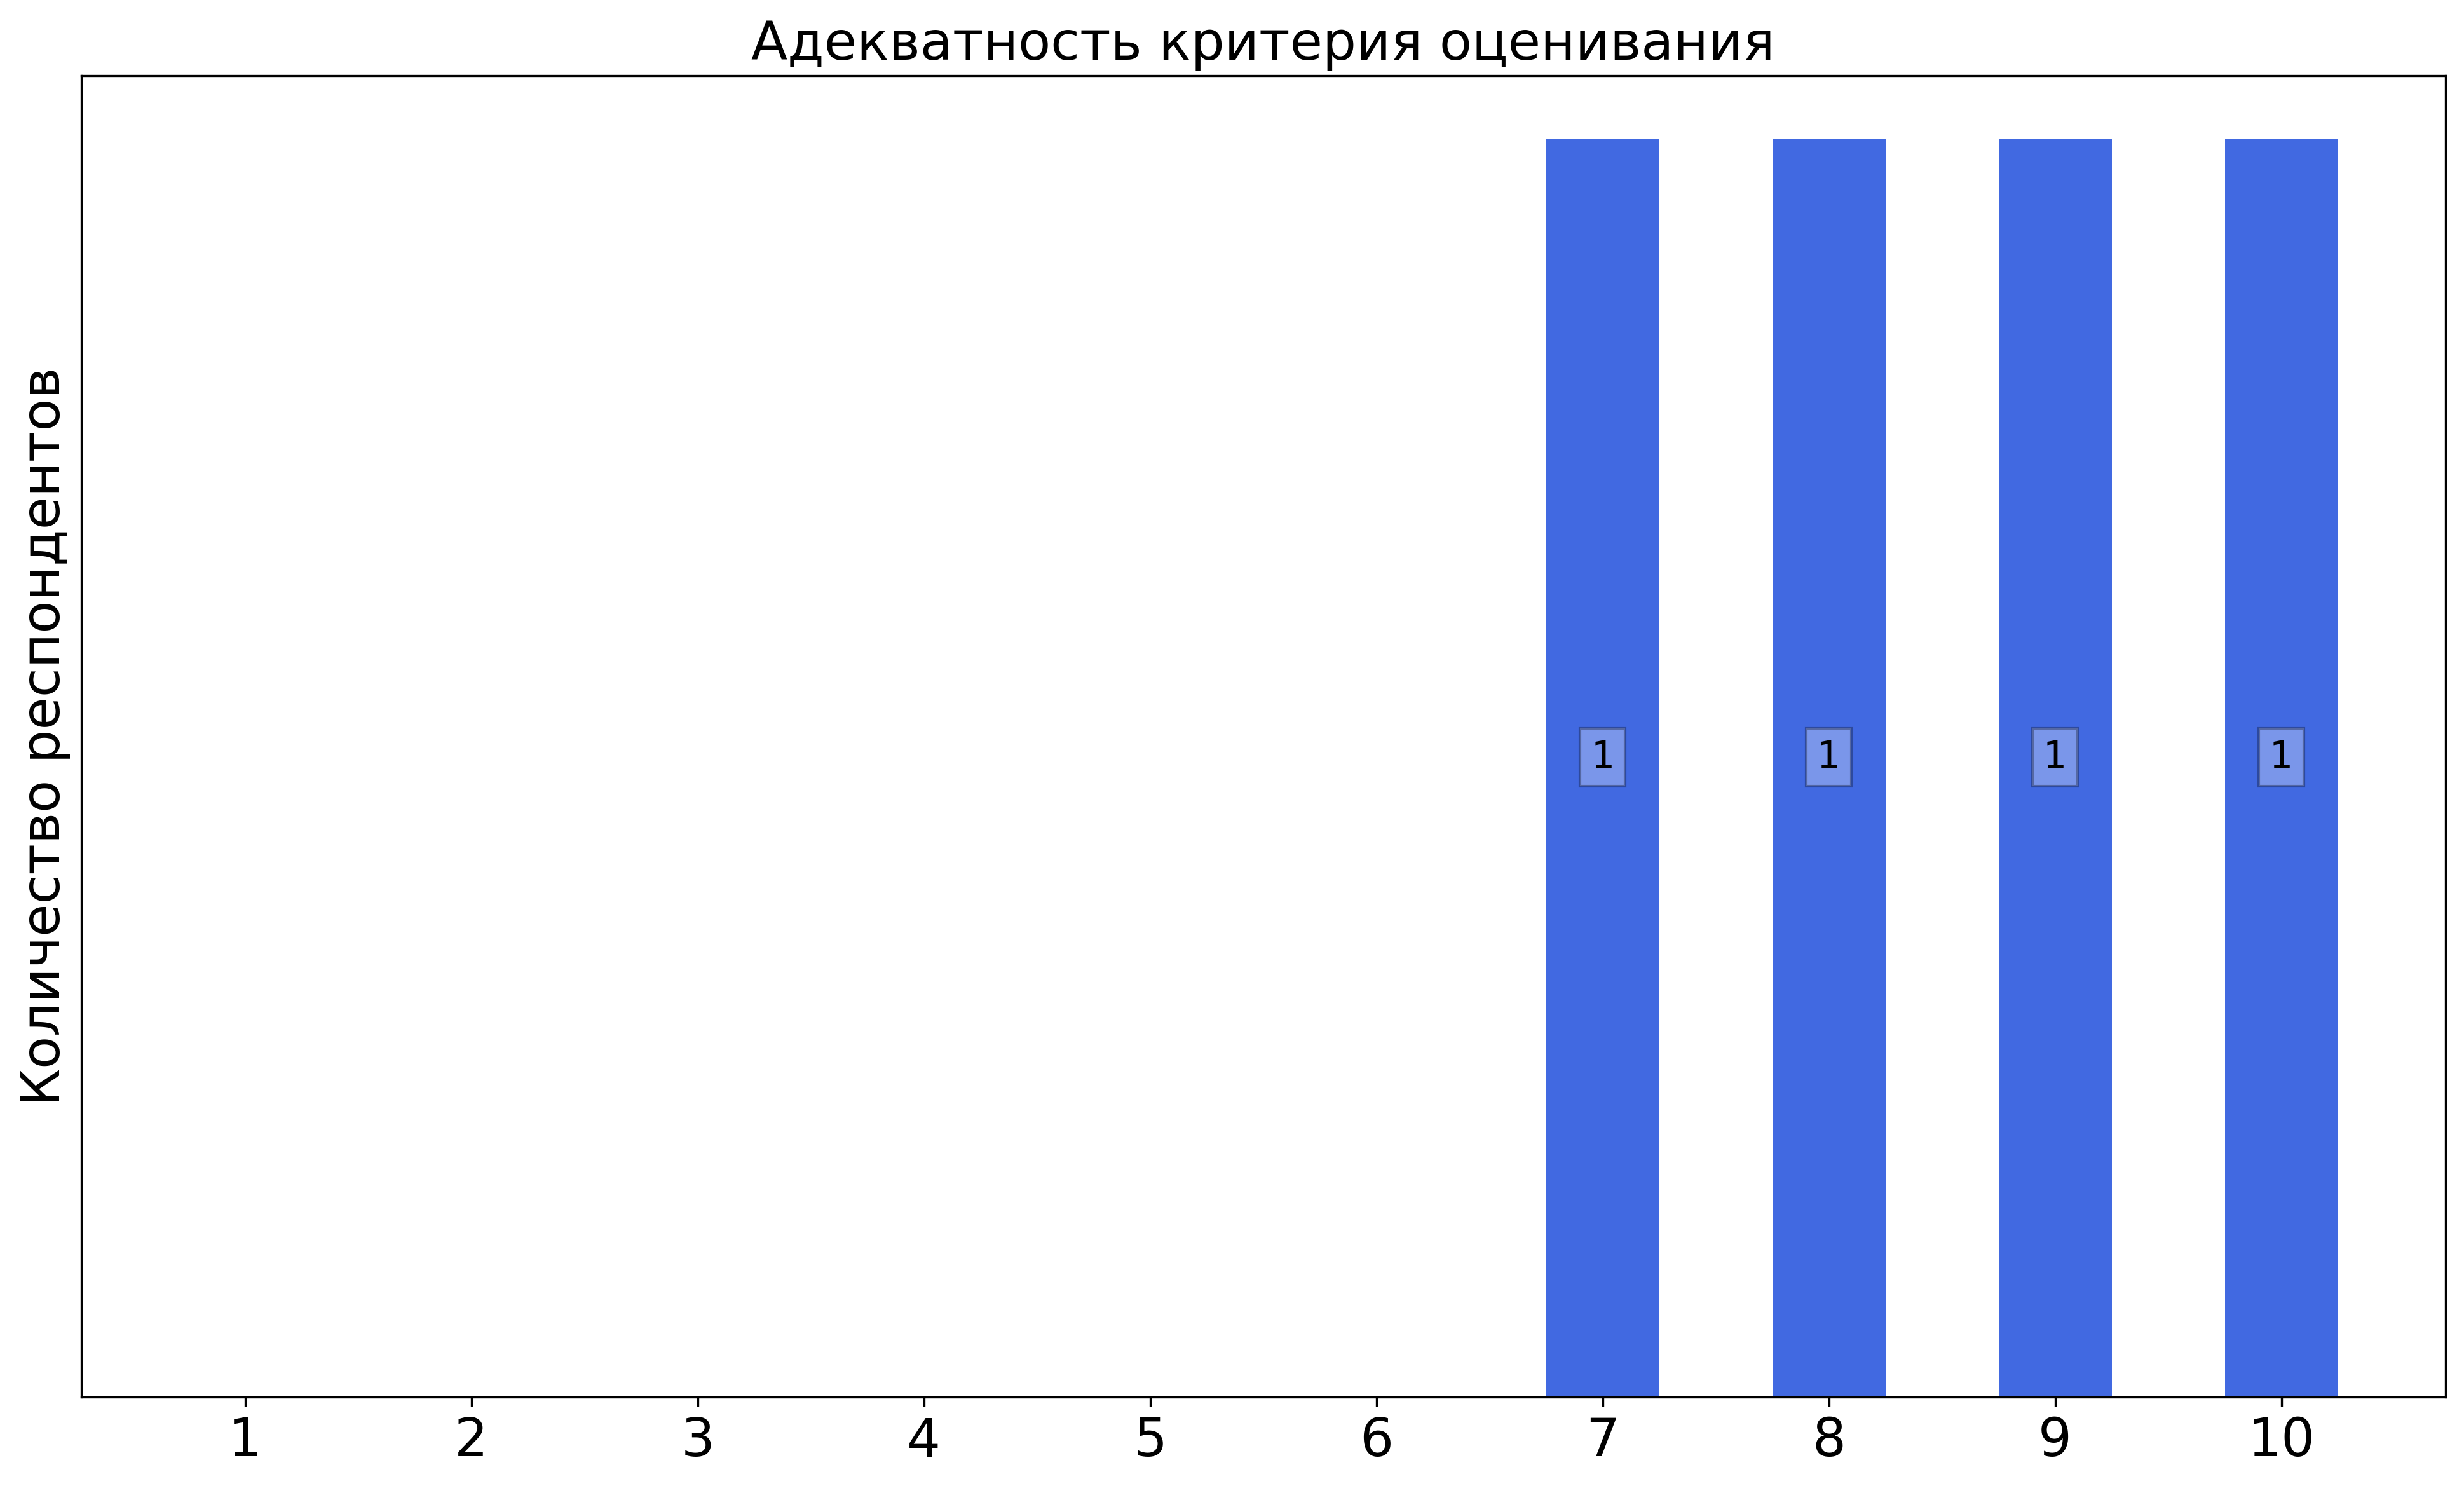
\includegraphics[width=\textwidth]{images/3 course/Лаборатория инфокоммуникационных технологий/labniks-marks-NetCracker-1.png}
            \end{subfigure}
            \begin{subfigure}[b]{0.45\textwidth}
                \centering
                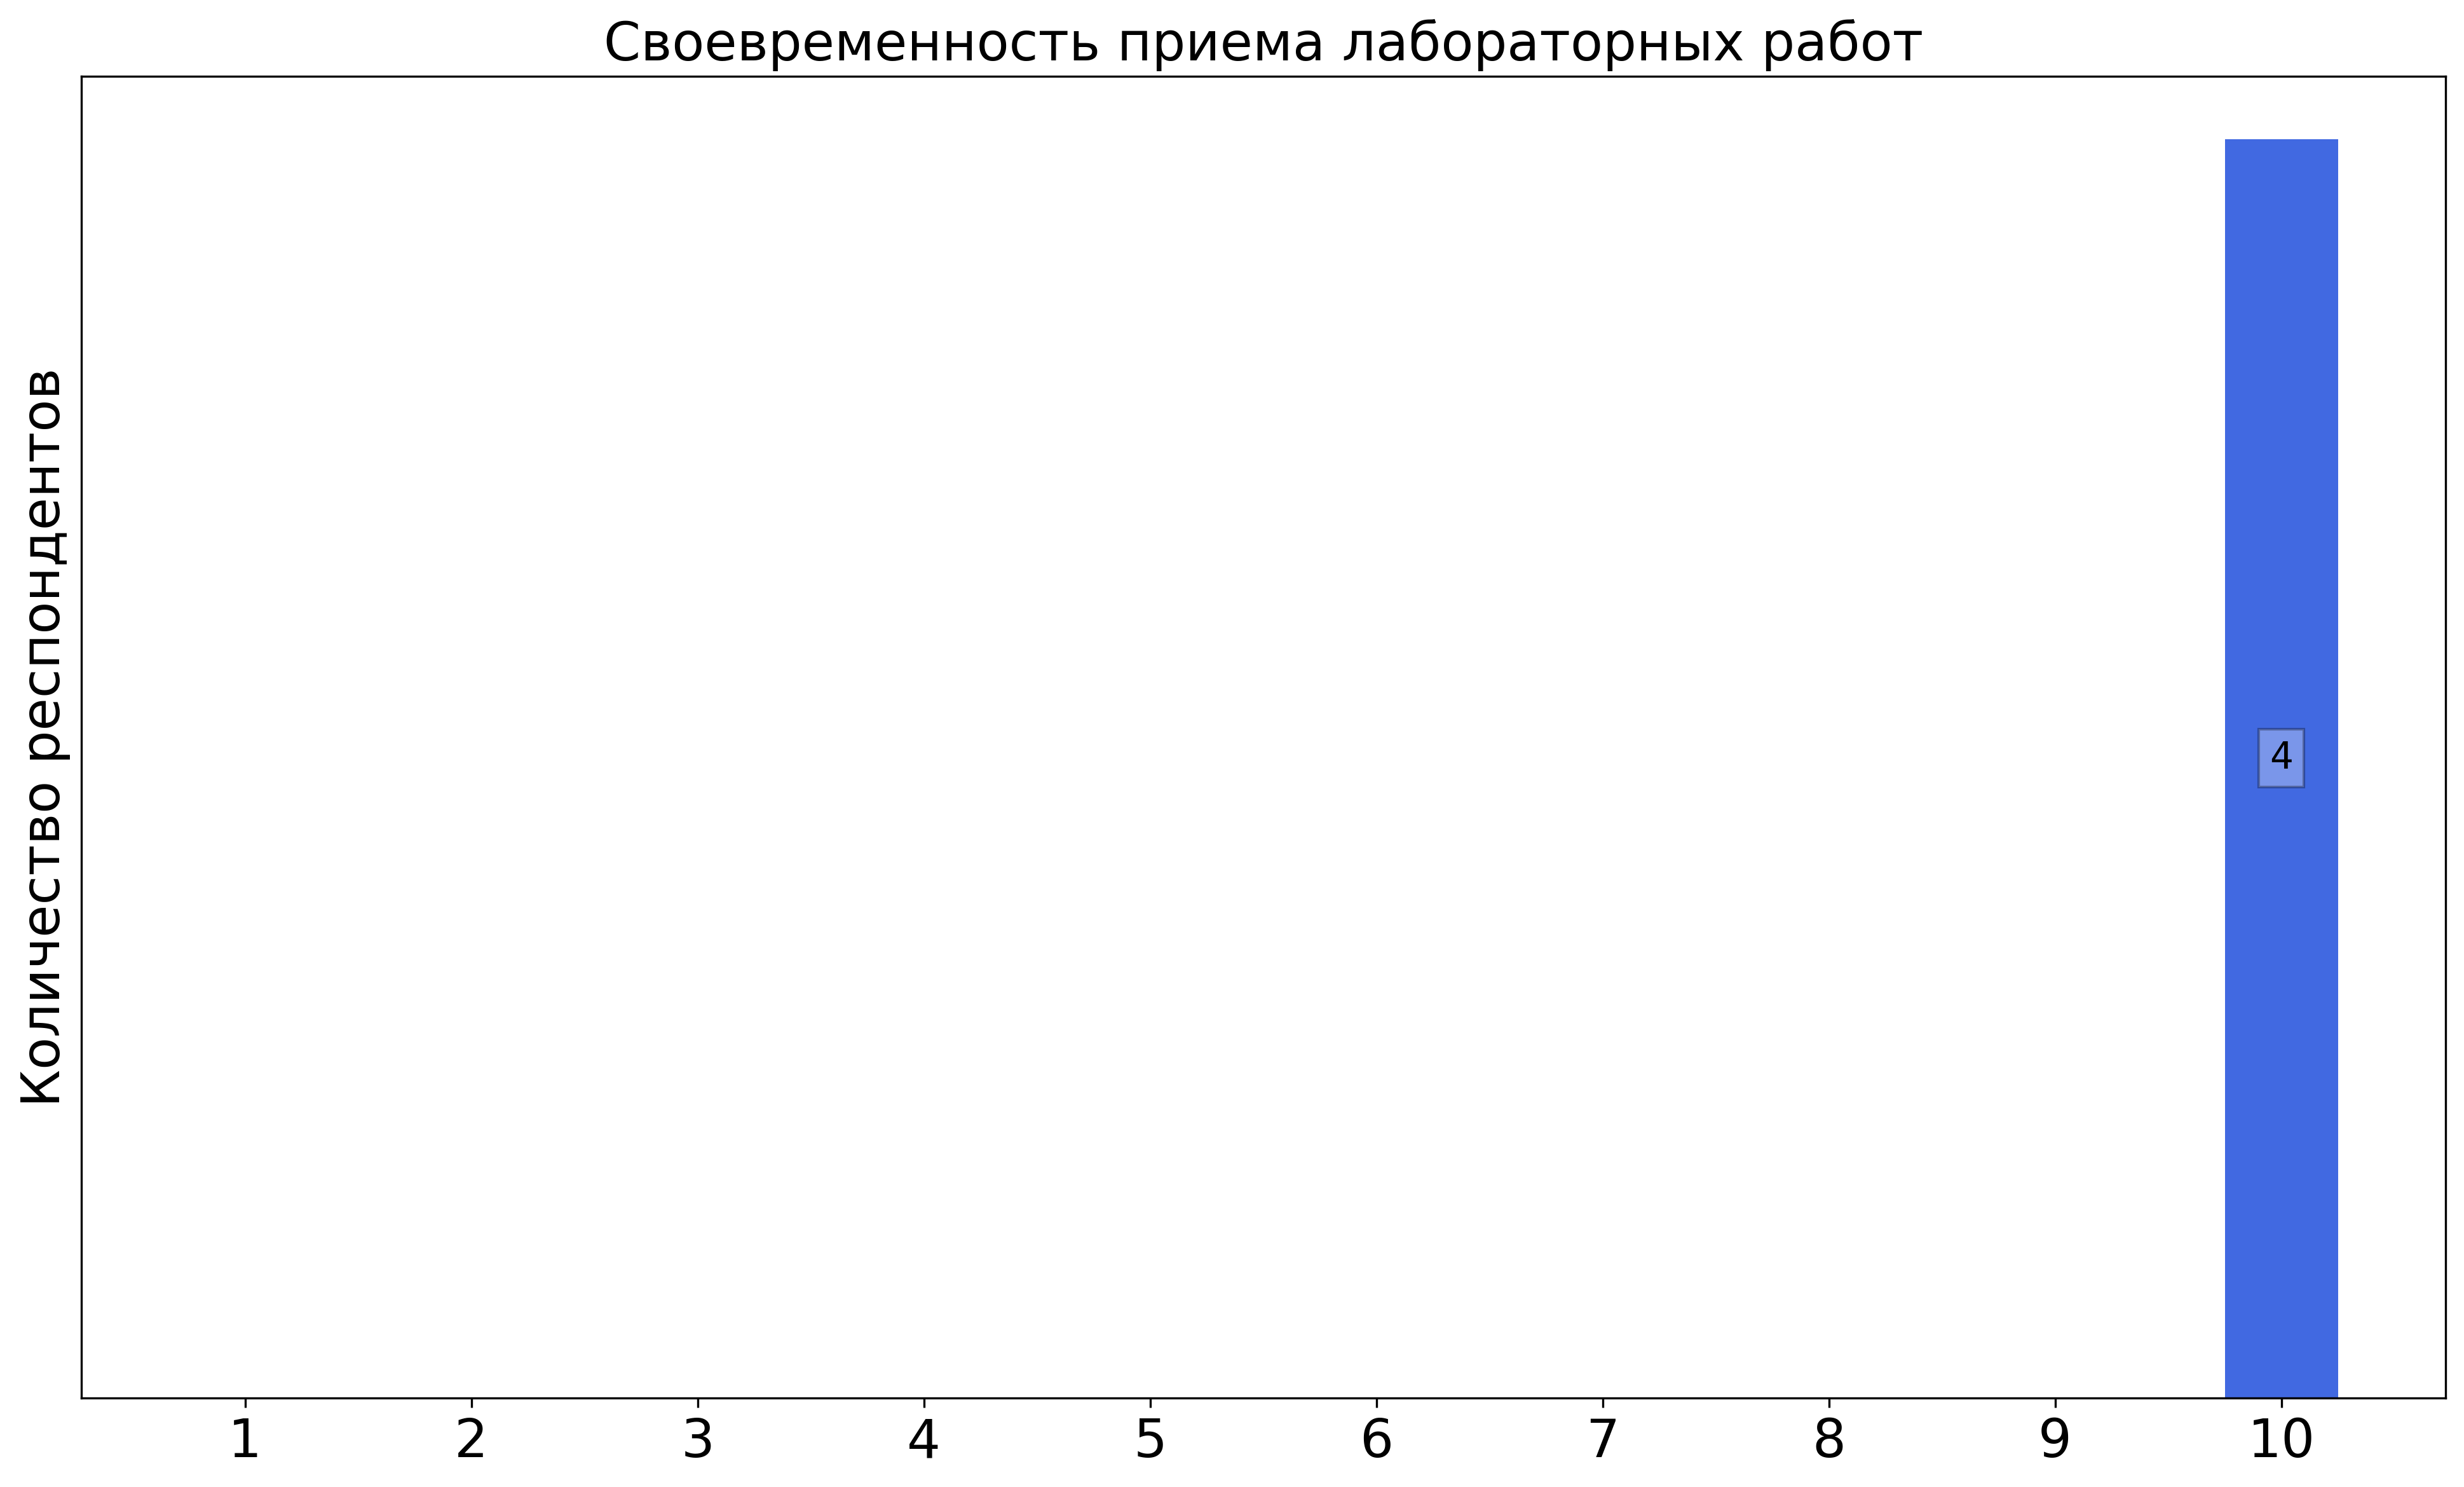
\includegraphics[width=\textwidth]{images/3 course/Лаборатория инфокоммуникационных технологий/labniks-marks-NetCracker-2.png}
            \end{subfigure}
            \begin{subfigure}[b]{0.45\textwidth}
                \centering
                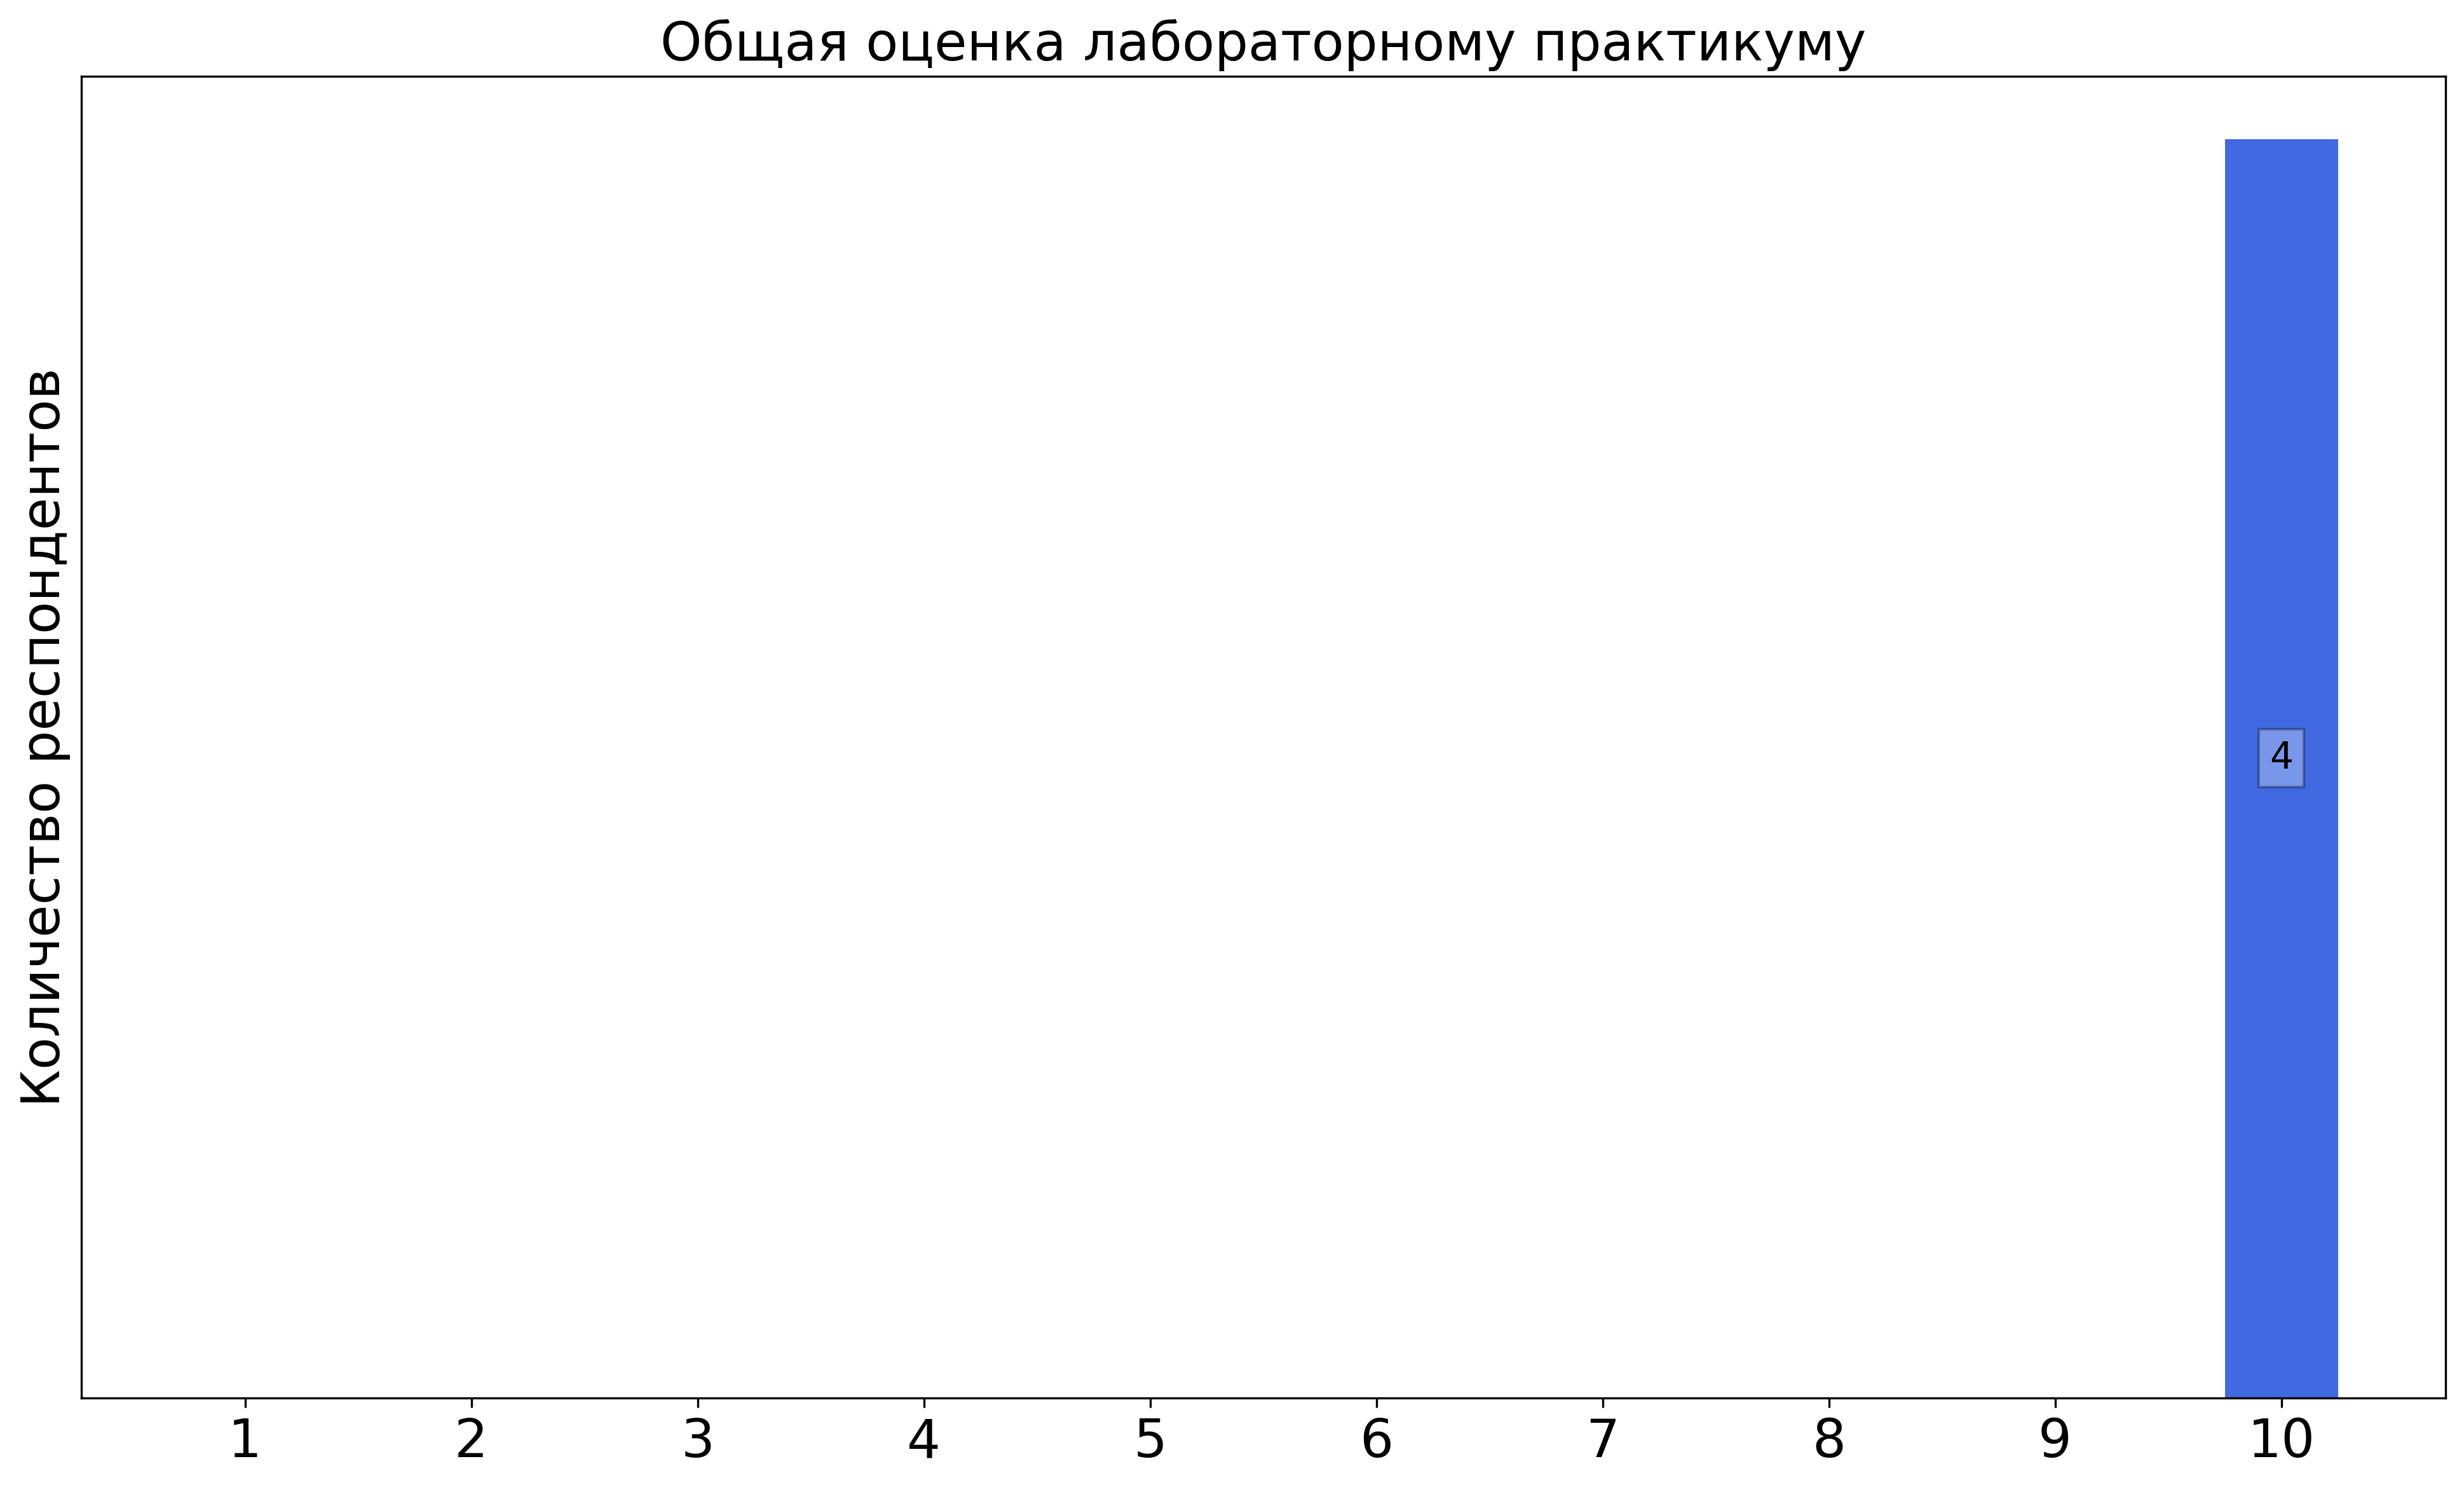
\includegraphics[width=\textwidth]{images/3 course/Лаборатория инфокоммуникационных технологий/labniks-marks-NetCracker-3.png}
            \end{subfigure}	
            \caption{Оценки респондентов о качестве преподавания лабораторных работ}
        \end{figure}

        \textbf{Комментарии студентов о преподавателе\protect\footnote{сохранены оригинальные орфография и пунктуация}}
            \begin{commentbox} 
                У NetCracker было все на высшем уровне. 
            \end{commentbox} 
        
            \begin{commentbox} 
                Лабы топ, один из лучших предметов в семестре. Климанов и его команда реально хотят научить и дать знания. Но итоговый зачет немного странный в плане выставления итоговой оценки, в принципе как и итоговая кр Климанова на его лекциях. Но тут уже это распространяется только на студентов крекера, так что пусть будет как есть. 
            \end{commentbox} 
                

    \subsubsection{Прочие комментарии и предложения по улучшению курса}
        \begin{commentbox}
            Лабы по сетям: совершенно непонятно зачем изучать систему команд вендера ушедшего из России. Лабы устарели. Хочется более прикладного программирования. Отсюда и вытекает изменение лекций по сетям. Опять же добавить больше прикладных тем.(не изучать устаревшие протоколы..)
        \end{commentbox}

		\begin{commentbox}
			Про лабораторные всё сказал выше. Лекциями удовлетворен, кроме опозданий лектора
		\end{commentbox}

        \begin{commentbox}
			Ввести нормальные критерии оценивания. 
		\end{commentbox}

        \begin{commentbox}
			"Есть предложение при выставлении автомата учитывать оценку за лекции по Компьютерным сетям.

            Также хотелось бы видеть более разбирающихся в предмете преподавателей. И, конечно, с адекватными критериями оценивания."
		\end{commentbox}

        \begin{commentbox}
			Замените преподавателей на практикуме
		\end{commentbox}

        \begin{commentbox}
			Сделать критерии получения автомата по лабам адекватными, сократить теорию по курсу (например убрать никому не нужную информацию о разновидностях полировки оптоволокна, которую потом лектор спрашивает в летучке на лекции)
		\end{commentbox}

        \begin{commentbox}
			Курс сам по себе неплох, лекции так и вовсе отличные, но методы оценивания вызывают только боль и желание поскорее от этих предметом избавиться. 
		\end{commentbox}

        \begin{commentbox}
			"Начну с того, что у курса большой прогресс, видимо он никогда не был настолько хорош как в этом году. Лекции прекрасны, все же отмечу, что Климанов слишком долго и образно объясняет отдельные моменты материала, уделяя им все, а остальным тонкостям ничего. Возможно это оправданно. Но это не согласуется с оцениванием. Коротко говоря, нужно больше практики, но в рамках лабораторных работ получить её тяжеловато. Вся система с повышающим коэффициентом противоречит общефизтеховской системе брс, поскольку является манипуляцией статистикой, в этом не должно быть необходимости, потому что материал лекций достаточно подробен, и можно спрашивать по нему, а не на всю глубину профессиональной области. Тест больше похож на формат собеседования и характеризует скорее профессиональные чем академические навыки. Что и приводит к заниженным оценкам и возмущению лектора.

            Короче говоря, тест рассчитан на уровень выше, хоть и хорош, а в полной мере научиться его решать в рамках 1+2 времени курса не получается. Надеюсь, повышающий коэффициент это временное решение, и со временем курс станет выпускать еще более квалифицированных специалистов в области КС. Лично, знания курса уже приносят пользу, хоть по кафедре я и далек от сетей, что очень радует."
		\end{commentbox}

        \begin{commentbox}
			Курс в целом не для всех, не всем нужно так глубоко знать физ устройство кабелей и конкретного вендора. Мне кажется, что стоит больше рассказывать про более прикладное и применимое для программистов общего плана (например, сеть в Linux). 
		\end{commentbox}

        \begin{commentbox}
			Курс должен быть очень интересен и полезен большей части факультета, однако о нем ходят легенды даже у ребят с других факультетов, а количество неудов по нему выше, чем, наверное, по любому другому зачету/экзамену.
            Что же не так? Наверно, стоит пересмотреть критерии оценивания, методы проведения контрольных и организованность преподавательского состава. К программе вопросов никаких нет"
		\end{commentbox}

        \begin{commentbox}
			Климанов отличный преподаватель, но критерии его оценивания странны и жестоки. Опоздания и регулярные задерживания создают ощущение неуважения к студентам. По поводу этого нужно провести с Максим Михайлович диалог.

            Курс лабораторных работ мало что дает студентам, не собирающемся идти в сисадмины/сетевых администраторов. Также было бы хорошо уменьшить случайность оценки из-за одного теста - например, добавить промежуточный тест(ы)"
		\end{commentbox}

        \begin{commentbox}
			Разбор конкретных примеров настройки оборудование в CISCO packet tracer, а не перечитывание текста с презентаций улучшило бы курс лабораторных работ.
		\end{commentbox}

        \begin{commentbox}
			Как насчет того, чтобы лабораторные практикумы вел человек ХОТЯ БЫ с нормальной артикуляцией. Воспринимать новый материал, который говорят МОНОТОННЫМ ЗАИКАЮЩИМСЯ ГОЛОСОМ - невероятно тяжело.
		\end{commentbox}

        \begin{commentbox}
			Максим Климанов как лектор - очень хорошо разбирается в сетевых технологиях, но критерии оценивания его курса это просто ужас. Весь семестр он рассказывает сухую теорию, но на контрольных он дает задачи, которые никто не учил правильно решать и судит исключительно по правильности решенных задач, что является очень странным и диким. Сама контрольная проводится 40 минут, даже не час. Очень не свойственный физтеху формат ответов, чисто на заучивание материала. Половина потока слетело со стипендии, наверное это что-то должно показывать?Частые опоздания на лекции и контрольные. Я считаю, что это человека по-хорошему нужно отстранить от педагогической практики, так как он необычайно жесток на оценки, но знаний феерических его курс не оставляет…
		\end{commentbox}

        \begin{commentbox}
			Пожелания по курсу - это посмотреть на то, какой курс сетей у ФПМИ.ИВТсп. То, что делали мы - мягко говоря сомнительно. Добавьте проги, добавьте проекты, учите актуальному. 
		\end{commentbox}

        \begin{commentbox}
			Мне кажется единственный способ решить эти проблемы - заменить преподавателей. Люди с таким подходом не смогут ничему научить, какими знаниями они не обладали и какие бы эксклюзивные темы не затрагивали. 

            Я считаю, что в таких предметах, по которым нельзя перевестись, нужны люди, умеющие преподавать и относящиеся к студентам по-человечески."
		\end{commentbox}

        \begin{commentbox}
			Уменьшить строгость оценивания
		\end{commentbox}

        \begin{commentbox}
			Необходимо заменить лектора. Студенты физтеха ежедневно испытывают серьёзные умственные нагрузки, и так издеваться над студентами  непростительно. Я считаю, расписание составляется не просто так, а для того чтобы лекции и семинары читались в определённое время.
		\end{commentbox}

        \begin{commentbox}
			Курс отличный(для крекеров), единственное, желаю Климанову не опаздывать больше на кр, чтобы студенты не седели от ожидания казни. 
		\end{commentbox}

        \begin{commentbox}
			Курс хороший, но необходимо полностью пересмотреть критерии оценивания. Лабораторный практикум вообще нуждается в пересмотре
		\end{commentbox}

        \begin{commentbox}
			Курс лабораторных работ для всех групп, проходящих базовый вариант, просто нужно убрать, в нынешнем виде он абсолютно бесполезен для всех, так как не связан с деятельностью базовых кафедр ни коим образом. Курс лекций также бесполезен практически для всех, его следовало бы сделать обязательным лишь для кафедр, связанным с сетями. Преподаётся лекционный курс очень хорошо, но оценивается абсолютно неадекватно. Стоит просто сказать о том, что отличную оценку получили 6 человек из 150. Если бы на контрольных проверялись исключительно знания теории, а умение решать задачи, которые студенты впервые видят на самих контрольных, было бы лучше. Ну, и оценивать явно нужно лояльнее, чем сейчас, спрашивая действительно основные для курса вещи, а не различные хитрости.
		\end{commentbox}

        \begin{commentbox}
			Разбить лекционных курс на 2 семестра. Потому что такое количество материала нормально не усваевается даже если курс реально интересен (у меня было окно перед лекцией, в которое я читал конспект Климанова и все равно к концу семестра все заботать было не реально).
		\end{commentbox}

        \begin{commentbox}
			Сменить преподавателей по лабам, составить кастомные лабы по материалам курса (программа-симулятор cisco позволяет это сделать), на лабах не рассказывать теорию лекций, а пояснять за лабы. Лектора также сменить, на лекционных контрольных давать только то, что давалось на лекциях и не больше того.
		\end{commentbox}

        \begin{commentbox}
            Увеличение количества часов при неизменной программе, возможность выполнять лабы не на занятии
        \end{commentbox}

        \begin{commentbox}
            Лучше не ходить на лекции и изучать самому, но, к сожалению, из за пропуска лекций теряется немалая часть баллов. 

            Совершенно не согласен с тем как лектор проверяет кр.
            Проверяются задания контрольных так, что для получения балла нужно досконально верно расписать всё решение. Даже решения в нужном направлении и имеющие правильный ответ, но отклоняющиеся от решения лектора не принимаются. 

            ПРОШУ ВЫКЛАДЫВАТЬ ЗАДАНИЯ КОНТРОЛЬНЫХ И ИХ РЕШЕНИЯ ДЛЯ ПОДГОТОВКИ
            Даже после проверки, на апелляции, нельзя было увидеть решения контрольной, что мы писали.
        \end{commentbox}

        \begin{commentbox}
            Хотелось бы видеть протоколы более высокого уровня для общего развития.
        \end{commentbox}

        \begin{commentbox}
            Хотелось бы больше практики. Например, сейчас я знаю кучу теорию по различным протоколам, но у меня нет никакого представления как это применять в жизни (банально как настроить роутер из командной строки). Хотелось бы добавить в курс лекции больше практики и меньше бесполезной теории. И вместо лаб в пакет трейсере сделать лабы как у группы Неткрекера
        \end{commentbox}    

        \begin{commentbox}
            Перераспределить время курса, сконцентрироваться на протоколах более высокого уровня и прикладным знаниям, связанным с ними. Отбросить ненужные подробности про физический уровень и детальное устройство некоторых протоколов. Полностью пересмотреть механизм оценивания. Если уж и оставлять в контрольных задачи - тогда выделить время на семинарах (cisco-лабах) для решения подобных задач.
        \end{commentbox}
